% First draft of the journal paper (tentative target: Computers & Chemical Engineering).
% Design: docs/superpowers/specs/2026-11-16-cace-paper-design.md. Plan: docs/superpowers/plans/2026-11-16-cace-paper.md.
% Build: latexmk in this directory (latexmkrc: pdflatex + bibtex).
% Numbers: every number in the text is a macro of numbers.tex, generated by make_numbers.py from the result JSON files.
%          Do not type numbers by hand; run `python3 make_numbers.py` after the JSON files change.
% Items for the authors to decide are marked with \todo{...} (red).
\documentclass[preprint,review,12pt]{elsarticle}

\usepackage{amsmath,amssymb}
\usepackage{booktabs}
\usepackage{graphicx}
\usepackage{lineno}
\usepackage{xcolor}
\usepackage{fvextra}
\usepackage{hyperref}

\newcommand{\todo}[1]{\textcolor{red}{[TODO: #1]}}
\newcommand{\Top}{\mathrm{Top}}
% Generated by make_numbers.py from the result JSON files. Do not edit by hand.
% Regenerate: python3 paper/cace/make_numbers.py
\newcommand{\AucCandDomAgree}{0.764}
\newcommand{\AucCandDomAgreeSE}{0.004}
\newcommand{\AucCandDomMatch}{0.573}
\newcommand{\AucCandDomMatchSE}{0.003}
\newcommand{\AucCandIoJac}{0.995}
\newcommand{\AucCandIoJacSE}{0.000}
\newcommand{\AucCandLatent}{0.909}
\newcommand{\AucCandLatentSE}{0.003}
\newcommand{\AucCandSpec}{0.994}
\newcommand{\AucCandSpecSE}{0.000}
\newcommand{\AucCandText}{0.849}
\newcommand{\AucCandTextSE}{0.005}
\newcommand{\AucFullDomAgree}{0.769}
\newcommand{\AucFullDomAgreeSE}{0.004}
\newcommand{\AucFullDomMatch}{0.577}
\newcommand{\AucFullDomMatchSE}{0.003}
\newcommand{\AucFullIoJac}{0.999}
\newcommand{\AucFullIoJacSE}{0.000}
\newcommand{\AucFullLatent}{0.948}
\newcommand{\AucFullLatentSE}{0.003}
\newcommand{\AucFullSpec}{0.999}
\newcommand{\AucFullSpecSE}{0.000}
\newcommand{\AucFullText}{0.909}
\newcommand{\AucFullTextSE}{0.004}
\newcommand{\BasePairFirst}{(1.0, 0.0)}
\newcommand{\BasePairLast}{(0.0, 1.0)}
\newcommand{\BaseValRecALowMax}{0.906}
\newcommand{\BaseValRecALowMin}{0.889}
\newcommand{\BaseValRecATextOnly}{0.362}
\newcommand{\BatchSize}{16}
\newcommand{\BmB}{0.75}
\newcommand{\BmKOne}{1.5}
\newcommand{\CopiesPerListOpus}{3.3}
\newcommand{\CopiesPerListProp}{3.3}
\newcommand{\CostHaiku}{255.23}
\newcommand{\CostOpus}{1{,}058.93}
\newcommand{\CostPerCallHaiku}{0.05}
\newcommand{\CostPerCallOpus}{0.21}
\newcommand{\CostTotal}{1{,}314.16}
\newcommand{\CovAFifty}{0.966}
\newcommand{\CovAFiveHundred}{0.998}
\newcommand{\CovATwoHundred}{0.992}
\newcommand{\DiffMapAEight}{+0.032}
\newcommand{\DiffMapAGreedyInfer}{+0.002}
\newcommand{\DiffMapAInferProp}{+0.013}
\newcommand{\DiffMapAPropBase}{+0.169}
\newcommand{\DiffMapATotal}{+0.169}
\newcommand{\DiffMapBEight}{+0.032}
\newcommand{\DiffMapBGreedyInfer}{+0.005}
\newcommand{\DiffMapBInferProp}{+0.012}
\newcommand{\DiffMapBPropBase}{+0.205}
\newcommand{\DiffMapCoh}{+0.074}
\newcommand{\DiffMapComp}{+0.073}
\newcommand{\DiffMapDomAgree}{+0.011}
\newcommand{\DiffMapSpec}{+0.099}
\newcommand{\DiffMapStepThree}{+0.073}
\newcommand{\DiffMapStepTwo}{+0.098}
\newcommand{\DiffRPrecAEight}{+0.056}
\newcommand{\DiffRPrecBEight}{+0.057}
\newcommand{\DiffRecAEight}{+0.010}
\newcommand{\DiffRecAPropBase}{+0.075}
\newcommand{\DiffRecATotal}{+0.074}
\newcommand{\DiffRecBEight}{+0.014}
\newcommand{\DiffRecBPropBase}{+0.141}
\newcommand{\DiffRecDomAgree}{-0.001}
\newcommand{\DiffRecDomMatch}{-0.008}
\newcommand{\DiffRecInHigh}{+0.186}
\newcommand{\DiffRecInLow}{+0.011}
\newcommand{\DiffRecKFive}{+0.094}
\newcommand{\DiffRecKTen}{+0.238}
\newcommand{\DiffRecKTwo}{+0.007}
\newcommand{\DiffRecLatent}{-0.021}
\newcommand{\DiffRecMergeBest}{-0.023}
\newcommand{\DiffRecMergeWorst}{-0.030}
\newcommand{\DiffRecSpec}{+0.068}
\newcommand{\DiffRecStepThree}{+0.006}
\newcommand{\DiffRecStepTwo}{+0.071}
\newcommand{\Dropout}{0.1}
\newcommand{\Epochs}{15}
\newcommand{\ErrRecall}{0.974}
\newcommand{\FirstSeed}{42}
\newcommand{\GapMapTwAHaikuBase}{0.380}
\newcommand{\GapMapTwAHaikuProp}{0.558}
\newcommand{\GapMapTwAOpusBase}{0.082}
\newcommand{\GapMapTwAOpusProp}{0.096}
\newcommand{\GapMapTwBHaikuBase}{0.288}
\newcommand{\GapMapTwBHaikuProp}{0.510}
\newcommand{\GapMapTwBOpusBase}{0.143}
\newcommand{\GapMapTwBOpusProp}{0.079}
\newcommand{\GapRecAHaikuBase}{0.409}
\newcommand{\GapRecAHaikuProp}{0.484}
\newcommand{\GapRecAOpusBase}{0.018}
\newcommand{\GapRecAOpusProp}{0.057}
\newcommand{\GapRecBHaikuBase}{0.293}
\newcommand{\GapRecBHaikuProp}{0.434}
\newcommand{\GapRecBOpusBase}{0.074}
\newcommand{\GapRecBOpusProp}{0.067}
\newcommand{\HaikuInvalidId}{31}
\newcommand{\HaikuOverTwenty}{645}
\newcommand{\HaikuRefusals}{144}
\newcommand{\HaikuRepeatedId}{626}
\newcommand{\HaikuWithTwenty}{4{,}412}
\newcommand{\Hidden}{64}
\newcommand{\JacBoth}{0.22}
\newcommand{\JacOnlyOpus}{0.17}
\newcommand{\JaccardHaiku}{0.324}
\newcommand{\JaccardOpus}{0.573}
\newcommand{\LearnRate}{10^{-3}}
\newcommand{\LiftMapKMax}{+0.095}
\newcommand{\LiftMapKMin}{+0.068}
\newcommand{\LiftMapKOne}{+0.007}
\newcommand{\MapABase}{0.693}
\newcommand{\MapABaseSD}{0.061}
\newcommand{\MapABm}{0.689}
\newcommand{\MapABmSD}{0.057}
\newcommand{\MapAEFive}{0.677}
\newcommand{\MapAEFiveSD}{0.058}
\newcommand{\MapAEightGreedy}{0.822}
\newcommand{\MapAEightInfer}{0.816}
\newcommand{\MapAEightProp}{0.790}
\newcommand{\MapAGreedy}{0.877}
\newcommand{\MapAGreedySD}{0.048}
\newcommand{\MapAInfer}{0.875}
\newcommand{\MapAInferSD}{0.046}
\newcommand{\MapAProp}{0.862}
\newcommand{\MapAPropSD}{0.053}
\newcommand{\MapARSeven}{0.789}
\newcommand{\MapARTwo}{0.691}
\newcommand{\MapASameW}{0.693}
\newcommand{\MapASpec}{0.790}
\newcommand{\MapBBase}{0.626}
\newcommand{\MapBBaseSD}{0.035}
\newcommand{\MapBBm}{0.622}
\newcommand{\MapBBmSD}{0.033}
\newcommand{\MapBEFive}{0.610}
\newcommand{\MapBEFiveSD}{0.029}
\newcommand{\MapBEightGreedy}{0.816}
\newcommand{\MapBEightInfer}{0.806}
\newcommand{\MapBEightProp}{0.785}
\newcommand{\MapBGreedy}{0.849}
\newcommand{\MapBGreedySD}{0.035}
\newcommand{\MapBInfer}{0.844}
\newcommand{\MapBInferSD}{0.036}
\newcommand{\MapBProp}{0.832}
\newcommand{\MapBPropSD}{0.041}
\newcommand{\MapKOneBase}{0.934}
\newcommand{\MapKOneProp}{0.931}
\newcommand{\MapTwABase}{0.680}
\newcommand{\MapTwABaseSD}{0.063}
\newcommand{\MapTwABm}{0.676}
\newcommand{\MapTwABmSD}{0.059}
\newcommand{\MapTwAEFive}{0.663}
\newcommand{\MapTwAEFiveSD}{0.059}
\newcommand{\MapTwAGreedy}{0.873}
\newcommand{\MapTwAGreedySD}{0.050}
\newcommand{\MapTwAHaiku}{0.300}
\newcommand{\MapTwAHaikuSD}{0.050}
\newcommand{\MapTwAInfer}{0.870}
\newcommand{\MapTwAInferSD}{0.048}
\newcommand{\MapTwAOpus}{0.761}
\newcommand{\MapTwAOpusSD}{0.063}
\newcommand{\MapTwAProp}{0.857}
\newcommand{\MapTwAPropSD}{0.055}
\newcommand{\MapTwBBase}{0.601}
\newcommand{\MapTwBBaseSD}{0.037}
\newcommand{\MapTwBBm}{0.596}
\newcommand{\MapTwBBmSD}{0.035}
\newcommand{\MapTwBEFive}{0.584}
\newcommand{\MapTwBEFiveSD}{0.030}
\newcommand{\MapTwBGreedy}{0.842}
\newcommand{\MapTwBGreedySD}{0.038}
\newcommand{\MapTwBHaiku}{0.313}
\newcommand{\MapTwBHaikuSD}{0.027}
\newcommand{\MapTwBInfer}{0.836}
\newcommand{\MapTwBInferSD}{0.039}
\newcommand{\MapTwBOpus}{0.744}
\newcommand{\MapTwBOpusSD}{0.044}
\newcommand{\MapTwBProp}{0.823}
\newcommand{\MapTwBPropSD}{0.044}
\newcommand{\MapTwCrossBase}{0.720}
\newcommand{\MapTwCrossBaseSD}{0.077}
\newcommand{\MapTwCrossHaiku}{0.237}
\newcommand{\MapTwCrossHaikuSD}{0.074}
\newcommand{\MapTwCrossOpus}{0.756}
\newcommand{\MapTwCrossOpusSD}{0.084}
\newcommand{\MapTwCrossProp}{0.886}
\newcommand{\MapTwCrossPropSD}{0.059}
\newcommand{\MapTwSingleBase}{0.942}
\newcommand{\MapTwSingleBaseSD}{0.042}
\newcommand{\MapTwSingleHaiku}{0.462}
\newcommand{\MapTwSingleHaikuSD}{0.054}
\newcommand{\MapTwSingleOpus}{0.922}
\newcommand{\MapTwSingleOpusSD}{0.052}
\newcommand{\MapTwSingleProp}{0.953}
\newcommand{\MapTwSinglePropSD}{0.023}
\newcommand{\MapTwSynthBase}{0.630}
\newcommand{\MapTwSynthBaseSD}{0.054}
\newcommand{\MapTwSynthHaiku}{0.329}
\newcommand{\MapTwSynthHaikuSD}{0.043}
\newcommand{\MapTwSynthOpus}{0.752}
\newcommand{\MapTwSynthOpusSD}{0.054}
\newcommand{\MapTwSynthProp}{0.831}
\newcommand{\MapTwSynthPropSD}{0.058}
\newcommand{\Margin}{0.1}
\newcommand{\MaxKCross}{3}
\newcommand{\MaxKSingle}{4}
\newcommand{\MaxKSynth}{10}
\newcommand{\MeanInSolved}{14.1}
\newcommand{\MeanInUnsolved}{25.8}
\newcommand{\MeanKAll}{3.99}
\newcommand{\MeanKCross}{2.01}
\newcommand{\MeanKSingle}{1.33}
\newcommand{\MeanKSolved}{3.55}
\newcommand{\MeanKSynth}{5.50}
\newcommand{\MeanKUnsolved}{7.81}
\newcommand{\MeanSrcCross}{2.01}
\newcommand{\MeanSrcSingle}{1.00}
\newcommand{\MeanSrcSynth}{1.10}
\newcommand{\NBasePairs}{12}
\newcommand{\NBothEq}{177}
\newcommand{\NCalls}{5{,}019}
\newcommand{\NCases}{1{,}731}
\newcommand{\NCross}{640}
\newcommand{\NCrossPicked}{33}
\newcommand{\NCrossProgram}{496}
\newcommand{\NCrossReselected}{111}
\newcommand{\NDbTokens}{952{,}144}
\newcommand{\NDistinctA}{1{,}586}
\newcommand{\NEarly}{39}
\newcommand{\NEarlyHand}{24}
\newcommand{\NEarlySearch}{15}
\newcommand{\NEq}{11{,}146}
\newcommand{\NEqPdf}{10{,}476}
\newcommand{\NEqRef}{670}
\newcommand{\NErrCases}{407}
\newcommand{\NErrGt}{1{,}622}
\newcommand{\NExcluded}{92}
\newcommand{\NExcludedCross}{91}
\newcommand{\NExtractEarliest}{9}
\newcommand{\NExtractPro}{320}
\newcommand{\NFields}{32}
\newcommand{\NGtAll}{6{,}910}
\newcommand{\NLabels}{1{,}998}
\newcommand{\NMeaningCases}{596}
\newcommand{\NMissed}{84}
\newcommand{\NNeg}{8}
\newcommand{\NOne}{2{,}000}
\newcommand{\NOneAllGt}{1{,}880}
\newcommand{\NOneOtherMax}{6{,}000}
\newcommand{\NOneOtherMin}{2{,}000}
\newcommand{\NOnlyOpusEq}{58}
\newcommand{\NOpenAlex}{290}
\newcommand{\NOpusLossMap}{843}
\newcommand{\NOpusLossRec}{486}
\newcommand{\NOpusTieMap}{469}
\newcommand{\NOpusTieRec}{1{,}064}
\newcommand{\NOpusWinCopies}{28}
\newcommand{\NOpusWinMap}{274}
\newcommand{\NOpusWinRec}{36}
\newcommand{\NOpusWinSevenPlus}{26}
\newcommand{\NPdf}{329}
\newcommand{\NPerFieldMax}{10}
\newcommand{\NPerFieldMin}{7}
\newcommand{\NPerm}{20}
\newcommand{\NRecEightA}{698}
\newcommand{\NRecEightB}{753}
\newcommand{\NRecordsA}{4{,}229}
\newcommand{\NRefSets}{32}
\newcommand{\NReqThreeTrivial}{1{,}724}
\newcommand{\NSearchPdf}{306}
\newcommand{\NSingle}{91}
\newcommand{\NSolved}{365}
\newcommand{\NSources}{361}
\newcommand{\NSplitCandidates}{400}
\newcommand{\NSplitsAll}{20}
\newcommand{\NSplitsHard}{20}
\newcommand{\NSymbolCases}{1{,}299}
\newcommand{\NSymbols}{13{,}220}
\newcommand{\NSymbolsConflict}{4{,}208}
\newcommand{\NSymbolsShared}{6{,}374}
\newcommand{\NSynth}{1{,}000}
\newcommand{\NSynthOneSource}{959}
\newcommand{\NTaskTokens}{303}
\newcommand{\NTestAMax}{527}
\newcommand{\NTestAMin}{298}
\newcommand{\NTestBMax}{289}
\newcommand{\NTestBMin}{193}
\newcommand{\NTestCrossMax}{200}
\newcommand{\NTestCrossMin}{119}
\newcommand{\NTestDistinct}{1{,}673}
\newcommand{\NTestFirstSplit}{407}
\newcommand{\NTestSingleMax}{32}
\newcommand{\NTestSingleMin}{10}
\newcommand{\NTestSynthMax}{304}
\newcommand{\NTestSynthMin}{160}
\newcommand{\NTrainFirstSplit}{975}
\newcommand{\NUnsolved}{42}
\newcommand{\NValAMax}{349}
\newcommand{\NValAMin}{216}
\newcommand{\NValBMax}{263}
\newcommand{\NValBMin}{149}
\newcommand{\OpusInvalidId}{21}
\newcommand{\OpusOverTwenty}{31}
\newcommand{\OpusRefusals}{0}
\newcommand{\OpusRepeatedId}{75}
\newcommand{\OpusWithTwenty}{4{,}838}
\newcommand{\OutTokensHaiku}{1{,}150}
\newcommand{\OutTokensOpus}{876}
\newcommand{\PfiDropMapTopic}{0.015}
\newcommand{\PfiDropMapVar}{0.853}
\newcommand{\PfiDropRecTopic}{0.007}
\newcommand{\PfiDropRecVar}{0.963}
\newcommand{\PfiMapTopic}{0.847}
\newcommand{\PfiMapVar}{0.009}
\newcommand{\PfiRecSpec}{0.089}
\newcommand{\PfiRecTopic}{0.974}
\newcommand{\PfiRecVar}{0.018}
\newcommand{\RPrecABase}{0.607}
\newcommand{\RPrecABaseSD}{0.059}
\newcommand{\RPrecABm}{0.599}
\newcommand{\RPrecABmSD}{0.055}
\newcommand{\RPrecAEFive}{0.595}
\newcommand{\RPrecAEFiveSD}{0.053}
\newcommand{\RPrecAGreedy}{0.811}
\newcommand{\RPrecAGreedySD}{0.070}
\newcommand{\RPrecAInfer}{0.805}
\newcommand{\RPrecAInferSD}{0.064}
\newcommand{\RPrecAProp}{0.782}
\newcommand{\RPrecAPropSD}{0.070}
\newcommand{\RPrecBBase}{0.555}
\newcommand{\RPrecBBaseSD}{0.036}
\newcommand{\RPrecBBm}{0.553}
\newcommand{\RPrecBBmSD}{0.033}
\newcommand{\RPrecBEFive}{0.544}
\newcommand{\RPrecBEFiveSD}{0.027}
\newcommand{\RPrecBGreedy}{0.793}
\newcommand{\RPrecBGreedySD}{0.039}
\newcommand{\RPrecBInfer}{0.782}
\newcommand{\RPrecBInferSD}{0.040}
\newcommand{\RPrecBProp}{0.755}
\newcommand{\RPrecBPropSD}{0.042}
\newcommand{\RankBoth}{17}
\newcommand{\RankOneCrossOpus}{90}
\newcommand{\RankOneCrossProp}{58}
\newcommand{\RankOneSynthOpus}{91}
\newcommand{\RankOneSynthProp}{73}
\newcommand{\RankOnlyOpus}{50.5}
\newcommand{\ReadShareHaiku}{93.6}
\newcommand{\ReadShareOpus}{90.2}
\newcommand{\RecABase}{0.906}
\newcommand{\RecABaseSD}{0.020}
\newcommand{\RecABm}{0.905}
\newcommand{\RecABmSD}{0.019}
\newcommand{\RecAEFive}{0.892}
\newcommand{\RecAEFiveSD}{0.023}
\newcommand{\RecAFiveHundredCand}{0.981}
\newcommand{\RecAGreedy}{0.983}
\newcommand{\RecAGreedySD}{0.009}
\newcommand{\RecAHaiku}{0.497}
\newcommand{\RecAHaikuSD}{0.063}
\newcommand{\RecAInfer}{0.982}
\newcommand{\RecAInferSD}{0.009}
\newcommand{\RecAOpus}{0.924}
\newcommand{\RecAOpusSD}{0.018}
\newcommand{\RecAProp}{0.981}
\newcommand{\RecAPropSD}{0.010}
\newcommand{\RecARSeven}{0.975}
\newcommand{\RecARTwo}{0.904}
\newcommand{\RecASameW}{0.907}
\newcommand{\RecASpec}{0.973}
\newcommand{\RecBBase}{0.825}
\newcommand{\RecBBaseSD}{0.024}
\newcommand{\RecBBm}{0.819}
\newcommand{\RecBBmSD}{0.023}
\newcommand{\RecBEFive}{0.806}
\newcommand{\RecBEFiveSD}{0.020}
\newcommand{\RecBGreedy}{0.971}
\newcommand{\RecBGreedySD}{0.014}
\newcommand{\RecBHaiku}{0.532}
\newcommand{\RecBHaikuSD}{0.038}
\newcommand{\RecBInfer}{0.970}
\newcommand{\RecBInferSD}{0.015}
\newcommand{\RecBOpus}{0.899}
\newcommand{\RecBOpusSD}{0.013}
\newcommand{\RecBProp}{0.966}
\newcommand{\RecBPropSD}{0.016}
\newcommand{\RecCrossBase}{0.989}
\newcommand{\RecCrossBaseSD}{0.007}
\newcommand{\RecCrossHaiku}{0.385}
\newcommand{\RecCrossHaikuSD}{0.109}
\newcommand{\RecCrossOpus}{0.950}
\newcommand{\RecCrossOpusSD}{0.026}
\newcommand{\RecCrossProp}{1.000}
\newcommand{\RecCrossPropSD}{0.000}
\newcommand{\RecKOneBase}{1.000}
\newcommand{\RecKOneProp}{1.000}
\newcommand{\RecSingleBase}{1.000}
\newcommand{\RecSingleBaseSD}{0.000}
\newcommand{\RecSingleHaiku}{0.823}
\newcommand{\RecSingleHaikuSD}{0.047}
\newcommand{\RecSingleOpus}{0.964}
\newcommand{\RecSingleOpusSD}{0.033}
\newcommand{\RecSingleProp}{1.000}
\newcommand{\RecSinglePropSD}{0.000}
\newcommand{\RecSynthBase}{0.842}
\newcommand{\RecSynthBaseSD}{0.031}
\newcommand{\RecSynthHaiku}{0.546}
\newcommand{\RecSynthHaikuSD}{0.052}
\newcommand{\RecSynthOpus}{0.904}
\newcommand{\RecSynthOpusSD}{0.016}
\newcommand{\RecSynthProp}{0.967}
\newcommand{\RecSynthPropSD}{0.016}
\newcommand{\RefSize}{5}
\newcommand{\RescueJac}{0.33}
\newcommand{\RescueLatent}{0.46}
\newcommand{\RescueSpec}{0.52}
\newcommand{\RescueText}{0.47}
\newcommand{\RunSameHaiku}{40.9}
\newcommand{\RunSameOpus}{72.0}
\newcommand{\RunSdHaiku}{0.142}
\newcommand{\RunSdOpus}{0.042}
\newcommand{\SameListHaiku}{2.0}
\newcommand{\SameListOpus}{0.06}
\newcommand{\Seeds}{42, 123, 456, 789, 1024, 2024, 3141, 5926, 7777, 9999}
\newcommand{\ShareHaikuRefusals}{2.9}
\newcommand{\ShareHaikuWithTwenty}{87.9}
\newcommand{\ShareKTwoPlus}{90.4}
\newcommand{\ShareLabelsOnce}{27.9}
\newcommand{\ShareOpusRefusals}{0.0}
\newcommand{\ShareOpusWinRec}{2.3}
\newcommand{\ShareOpusWithTwenty}{96.4}
\newcommand{\StagePairs}{$(0.7, 0.3)$, $(0.5, 0.5)$, $(0.3, 0.7)$, and $(0.0, 1.0)$}
\newcommand{\SvdDim}{256}
\newcommand{\TerHighOpus}{0.769}
\newcommand{\TerHighProp}{0.922}
\newcommand{\TerHighWin}{5.8}
\newcommand{\TerLowOpus}{0.780}
\newcommand{\TerLowProp}{0.858}
\newcommand{\TerLowWin}{19.5}
\newcommand{\TerMidOpus}{0.773}
\newcommand{\TerMidProp}{0.924}
\newcommand{\TerMidWin}{8.0}
\newcommand{\TextBoth}{0.10}
\newcommand{\TextOnlyOpus}{0.07}
\newcommand{\TimeRatioA}{2.4}
\newcommand{\TimeRunA}{161}
\newcommand{\TimeRunAFifty}{66}
\newcommand{\ValRecAMax}{0.983}
\newcommand{\ValRecAMin}{0.980}
\newcommand{\ValRecBMax}{0.975}
\newcommand{\ValRecBMin}{0.974}
\newcommand{\VarsBoth}{7.0}
\newcommand{\VarsOnlyOpus}{5.4}
\newcommand{\WText}{0.3}
\newcommand{\WVar}{0.7}
\newcommand{\WeightDecay}{10^{-4}}
\newcommand{\WinsMapAGreedyInfer}{7}
\newcommand{\WinsMapBGreedyInfer}{9}
\newcommand{\WinsMapDomAgree}{9}
\newcommand{\WinsMapStepOne}{3}
\newcommand{\WinsMapStepThree}{10}
\newcommand{\WinsMapTwAHaikuBase}{0}
\newcommand{\WinsMapTwAHaikuProp}{0}
\newcommand{\WinsMapTwAOpusBase}{10}
\newcommand{\WinsMapTwAOpusProp}{0}
\newcommand{\WinsMapTwBHaikuBase}{0}
\newcommand{\WinsMapTwBHaikuProp}{0}
\newcommand{\WinsMapTwBOpusBase}{10}
\newcommand{\WinsMapTwBOpusProp}{0}
\newcommand{\WinsRecAEight}{9}
\newcommand{\WinsRecAHaikuBase}{0}
\newcommand{\WinsRecAHaikuProp}{0}
\newcommand{\WinsRecAOpusBase}{10}
\newcommand{\WinsRecAOpusProp}{0}
\newcommand{\WinsRecBEight}{9}
\newcommand{\WinsRecBHaikuBase}{0}
\newcommand{\WinsRecBHaikuProp}{0}
\newcommand{\WinsRecBOpusBase}{10}
\newcommand{\WinsRecBOpusProp}{0}
\newcommand{\WinsRecDomAgree}{3}
\newcommand{\WinsRecDomMatch}{5}
\newcommand{\WinsRecLatent}{3}
\newcommand{\WinsRecStepOne}{3}
\newcommand{\WinsRecStepThree}{9}
\newcommand{\WrongInIoOpus}{4.1}
\newcommand{\WrongInIoProp}{9.2}
\newcommand{\WrongInIoPropLoss}{8.6}
\newcommand{\WrongInIoPropTie}{8.1}


\journal{Computers \& Chemical Engineering}

\begin{document}

\begin{frontmatter}

\title{Equation-set retrieval using equations and context extracted from the literature for automated physical model building}

\author{\todo{authors, affiliations, and corresponding author}}

\begin{abstract}
Building a physical model for a process outside the libraries of modeling tools requires an
engineer to collect equations scattered across many documents and to assemble them into a model.
This study addresses one step of automating this work: given a description of the desired model and
its input and output variables, present the equations likely to serve in the model, drawn from a
database of equations extracted from the literature. Because an equation that contains a variable
other than the inputs and outputs is useful only together with an equation that determines that
variable, we propose a two-stage retrieval method that judges each candidate by its relation to
other equations. The first stage narrows the database by text similarity and variable overlap; the
second reranks the candidates with a multilayer perceptron that reads seven query--equation
features and three set-aware features. On a database of \NEq{} equations and \NCases{} cases split
by source, the method raised Recall@20, the fraction of the ground-truth equations among the 20
presented, from \RecABase{} for classical retrieval to \RecAProp, in all 10 splits. Ablation and
permutation importance show that the features reading the variables shared among equations cause
most of the gain, whereas topical similarity adds little. Two large language models that read the
whole database without training reached \RecAOpus{} and \RecAHaiku; the proposed method beat both
in every split. The larger model came close on models drawn from a single source and found
equations that share few variables with the query, at \CostPerCallOpus{} US dollars per query and
with answers that varied between runs.

\end{abstract}

\begin{highlights}
\item Highlights to be written.

\end{highlights}

\begin{keyword}
Physical model building \sep Equation retrieval

\end{keyword}

\end{frontmatter}

\linenumbers

\section{Introduction}\label{sec:intro}

Physical models, systems of equations that describe how the material, energy, and momentum of a
process change, underpin the process industry. Process design sizes equipment on them, process
control tunes controllers on them, and a digital twin keeps such a model in step with the running
plant \citep{DigitalTwin}. Tools such as MATLAB/Simulink \citep{simulink} and Aspen Plus
\citep{aspen} let an engineer assemble a model quickly, but only for the unit operations and
phenomena that their libraries cover. For a process outside those libraries, the engineer surveys
papers, textbooks, and handbooks, collects the equations scattered across them, and refines a
prototype model by trial and error. Modeling a new process is therefore slow, and it depends on the
few experts who can read the literature of the field.

To free engineers from this work, an automated physical model builder, AutoPMoB, has been proposed
\citep{AutoPMoBCSTR,AutoPMoBProto}. As Fig.~\ref{fig:overview}(a) shows, AutoPMoB collects
documents about a target process, extracts equations, variables, and experimental data from them,
judges which extracted items are equivalent across documents, and reorganizes the equivalent items
into the desired model. Its component technologies extract variable symbols and their definitions
\citep{VARAT,Nagayama}, judge whether two variable definitions refer to the same quantity
\citep{ProcessBERT}, judge whether two equation systems are equivalent \citep{DAEEquiv}, and
combine given equations into models that meet predefined requirements \citep{CombineEq}.

\begin{figure}[tbp]\centering
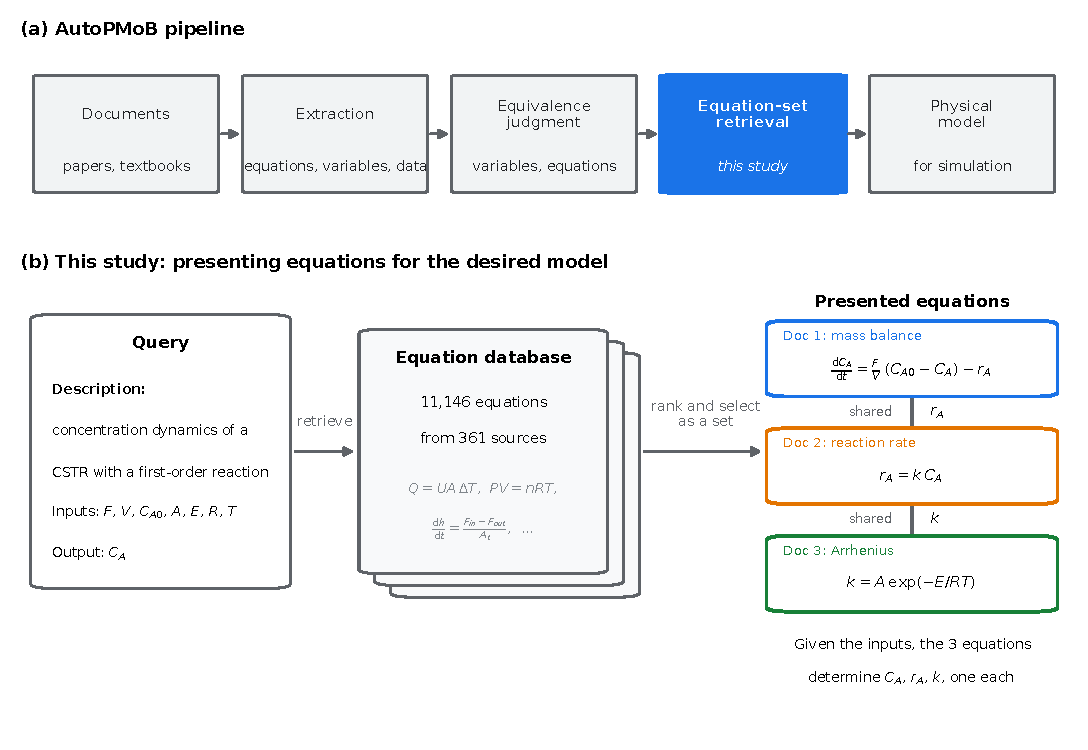
\includegraphics[width=0.98\linewidth]{figures/fig_autopmob_overview.pdf}
\caption{The automated physical model builder (AutoPMoB) and the position of this study. (a)
AutoPMoB collects documents about a target process, extracts equations, variables, and data,
judges their equivalence across documents, and reorganizes them into the desired model; this study
addresses the highlighted stage. (b) The task of this study: a query gives a description of the
desired model with its input and output variables, and the method presents, from a database of
equations extracted from many documents, the equations likely to serve in the model. The three
presented equations come from different documents and are linked by the variables they share
($r_A$ and $k$); once the inputs are given, they determine the three unknowns $C_A$, $r_A$, and
$k$, one equation each.}
\label{fig:overview}
\end{figure}

This study addresses the step that precedes the combination: given a description of the desired
model together with its input and output variables, present the equations likely to serve in the
model, drawn from a large equation database built from many documents
(Fig.~\ref{fig:overview}(b)). The aim is to present equations that are likely to be usable, not a
finished model; the engineer assembles and checks the model from them. The step is a retrieval
problem whose candidates depend on one another. A physical model is a set of equations from which
the output variables can be computed once the input variables are given, so an equation that
contains a variable other than the inputs and outputs is useful only together with an equation that
determines that variable. The concentration dynamics of a continuous stirred-tank reactor, for
example, need three equations: the mass-balance ordinary differential equation for the
concentration, the reaction-rate equation $r_A = k C_A$, and the Arrhenius equation
$k = A\exp(-E/RT)$ for the rate constant. The differential equation alone leaves the rate $r_A$
undetermined, the rate equation alone leaves the rate constant $k$ undetermined, and only the three
together determine the concentration from the inputs. A method that scores each equation by its
similarity to the description cannot see these dependencies. Retrieval must therefore evaluate
candidate equations as a set, not one by one.

We propose \ours{} (two-stage retrieval with attribute-conditioned evaluation). The first stage
ranks the whole database by a mixture of text similarity and variable overlap and keeps the top
candidates. The second stage evaluates each candidate again, conditioned on three attributes of an
equation: its variable set, its domain label, and its text. A multilayer perceptron reads ten
features of these attributes: seven compare a candidate with the query, and three, the set-aware
features, compare it with a reference set of equations. The set-aware features ask whether the
candidate supplies query variables that the reference set still lacks, whether it shares variables
with the set, and whether it carries the same domain label. A learned greedy variant builds the
ranking one equation at a time and compares each candidate with the equations already selected.

To evaluate the method, we built a database of \NEq{} equations: \NEqPdf{} that a large language
model (LLM) extracted from \NPdf{} PDF files of papers, textbooks, and reports, and \NEqRef{} that
it generated to cover textbook fundamentals. We also built \NCases{} cases, each a query with a
ground-truth equation set that meets the input--output and degree-of-freedom requirements of
\citet{CombineEq}. We split the cases by source into training,
validation, and test cases, repeat every experiment over 10 stratified splits, and choose the
hyperparameters on the validation cases.

\ours{} outperforms classical retrieval. Recall@20, the fraction of the ground-truth
equations among the 20 equations presented, rises from \RecABase{} to \RecAProp{} on all cases and
from \RecBBase{} to \RecBProp{} on the \NSynth{} cases that a program synthesized, in all 10 splits,
and the gain grows with the numbers of ground-truth equations and input variables. Ablation and
permutation importance locate the cause in the variables that the query and the equations share,
not in their topic.
We also compare the method with LLMs that receive the whole database and select equations without
training. The larger model, Claude Opus~5.5, reaches a Recall@20 of \RecAOpus{} and beats classical
retrieval, but \ours{} beats it in every split, by the widest margins on models that
combine several sources or many equations.

The contributions of this study are fourfold:
\begin{enumerate}
  \item a formulation of equation selection for physical model building as the retrieval of an
    equation set, with a benchmark of \NEq{} equations and \NCases{} cases split by source;
  \item \ours, a two-stage retrieval method with attribute-conditioned evaluation that improves
    Recall@20 and mean average precision over classical retrieval in every split;
  \item an empirical account of the method: which features cause the improvement, where
    sequential selection helps, why topical similarity adds little, and where the remaining errors
    arise;
  \item a comparison with LLMs that read the whole database, which identifies the strengths and
    weaknesses of the two approaches in accuracy, cost, and repeatability.
\end{enumerate}

\section{Related work}\label{sec:related}

\paragraph{Automated physical model building} AutoPMoB collects documents about a target process,
extracts equations, variables, and experimental data, judges the equivalence of the extracted
information across documents, and reorganizes it into the desired model
\citep{AutoPMoBCSTR,AutoPMoBProto}. For extraction, an annotation tool and an algorithm collect
variable symbols from engineering documents \citep{VARAT}, and template sentences augment the data
for extracting variable definitions \citep{Nagayama}. For equivalence judgment, ProcessBERT, a
language model pre-trained on a chemical-engineering corpus, judges whether two variable
definitions refer to the same quantity \citep{ProcessBERT}, and a computer-algebra algorithm judges
whether two groups of equations are equivalent \citep{DAEEquiv,ZhangEquiv}. The work closest to
this study addresses the model-building step itself: \citet{KatoESCAPE} proposed an algorithm that
builds a model from extracted equations, and \citet{CombineEq} formulated model building as the
combination of extracted equations into models that satisfy four predefined requirements and
proposed an algorithm that finds every such model. This study differs in its input and output. The
combination method takes equations and their variables and returns every combination that meets the
requirements. This study also takes a description of the desired model, reads a context text for
each equation, and ranks the equations that the description asks for above the rest. Finding the
equations that concern the requested model does not by itself require context: in our benchmark,
whose queries take their variables from the symbols of the ground-truth equations, variable overlap
decides most of the ranking (Section~\ref{sec:mechanism}). Context is needed where variables cannot
decide, as when several combinations meet the requirements and only the description tells which one
the user wants, and this study does not show that it helps there.

\paragraph{Equation discovery from numerical data} Symbolic regression searches for an equation
that fits numerical data, determining its form as well as its coefficients \citep{AIFeynman}.
\citet{SchmidtLipson} distilled conservation laws from motion-tracking data without prior knowledge
of physics, sparse identification of nonlinear dynamics keeps the fewest terms of the governing
equations that represent the data \citep{SINDy}, and ALAMO learns algebraic surrogate models that
are as accurate and as simple as possible from few simulations or experiments \citep{ALAMO}. The
difficulty lies in the search: the candidate forms span a very large combinatorial space, and
methods that learn from data alone leave unused the knowledge that scientists rely on. LLM-SR
brings that knowledge in by letting an LLM propose equation skeletons, whose parameters an
optimizer fits to the data \citep{LLMSR}. This study differs in where its equations come from: it
builds a model from equations collected from the literature, so it needs no data measured on the
target process, and it reads context, which numbers do not carry. The two approaches can work
together, because the retrieved equations, with their coefficients left free, can serve as
candidate skeletons for symbolic regression.

\paragraph{Information retrieval and reranking} Classical information retrieval ranks the items of
a collection by their relevance to a query \citep{Manning}: term-weighting schemes such as TF-IDF
score lexical overlap \citep{Salton}, BM25 refines such scores \citep{BM25}, and latent semantic
analysis absorbs vocabulary mismatch in a low-dimensional space \citep{LSA}. Modern systems add a
second stage, in which a learned model, today typically a pretrained language model, reranks the
candidates of a fast first-stage retriever \citep{BERT,BERTrerank}, and dense retrievers perform
the first stage with learned embeddings \citep{DPR}. Our method inherits this retrieve-then-rerank
design and trains its reranker with a pairwise ranking loss \citep{LTR}. These methods score each
item independently of the other retrieved items. The best-known departure, maximal marginal
relevance, penalizes a candidate for resembling the items already selected and thereby diversifies
the result list \citep{MMR}. Our task needs the opposite relation: a good candidate should connect
to the equations already selected, by sharing their variables, and supply the query variables they
still miss. Where maximal marginal relevance treats overlap as redundancy, equation-set retrieval
treats shared variables as the links that make the equations a system.

\paragraph{Generation by large language models} LLMs generate domain knowledge directly from a
prompt \citep{GPT3}, so asking an LLM to write out the equations of the desired model is a natural
alternative to retrieving them. Generation, however, carries no provenance: LLMs produce fluent
output that no source supports \citep{Hallucination}, and a user cannot trace a generated equation
to a source to check it. The check matters for physical models, whose equations are solved as one
system, so that a single wrong equation can corrupt every variable connected to it. An LLM can
instead select equations from a database, which keeps the link to the sources, and
Section~\ref{sec:llmresults} compares the proposed method with LLMs used in this way.

\paragraph{Mathematical information retrieval} Mathematical information retrieval searches for
formulas with queries that contain text, formulas, or both \citep{MathSurvey}. Its methods compare
formulas as strings of symbols, as operator trees whose paths are matched \citep{Approach0}, or as
embeddings of those trees \citep{TangentCFT}. For this study such methods are components, not
rivals: our second stage also compares equations, but it reads only the sets of variables that
they contain. Shared tasks such as NTCIR-12 MathIR \citep{NTCIR12} and ARQMath \citep{ARQMath}
retrieve single formulas ranked by similarity to the query. Our method presents equations meant to
be used together, so the value of one equation depends on the equations presented with it, and we
found no formula-search benchmark that imposes this joint condition.

\section{Problem formulation}\label{sec:formulation}
The requirements follow \citet{CombineEq}.

\section{Method}\label{sec:method}

The method works in two stages. The first stage scores every equation of the database on its own
and keeps the best as candidates. The second stage reranks the candidates with a learned model that
compares each candidate with other equations.

\subsection{Stage 1: candidate retrieval}\label{sec:stage1}

The first stage keeps the $N_1$ equations with the highest score as the candidate set $C_q$. The
score mixes one text term and one variable term,
\begin{equation}
  s_1(q, e_j) = w_{\mathrm{t}} \cos\!\big(\mathrm{tfidf}(c), \mathrm{tfidf}(t_j)\big)
              + w_{\mathrm{v}} \, J\!\big(\mathcal{Q}, V(e_j)\big) ,
  \label{eq:stage1}
\end{equation}
where $t_j$ joins the context text, the expression, and the domain label of equation $e_j$. The
first term, the text similarity, compares the description with this text through
term-frequency--inverse-document-frequency (TF-IDF) vectors \citep{Salton} over word unigrams and
bigrams. The second term, the variable overlap, is the Jaccard similarity
$J(A, B) = |A \cap B| / |A \cup B|$ between the query variables and the variables of the equation.
Ranking the whole database by Eq.~\eqref{eq:stage1} is a classical information-retrieval method
\citep{Manning}, and Section~\ref{sec:setup} uses it, without a learned model or a candidate set,
as the baseline.

The second stage reranks only the candidates, so the fraction of ground-truth equations among them,
the candidate coverage, bounds what the second stage can achieve. We set $N_1$ so large that every
ground-truth equation enters the candidates (Section~\ref{sec:compared}).

\subsection{Stage 2: set-aware reranking}\label{sec:stage2}

The second stage judges each candidate against the equations already at hand.
Table~\ref{tab:features} lists its ten features. Seven compare the query with a single equation:
two measure the topical closeness of the description ($f_1$, $f_3$), one matches the domain label
against the description ($f_7$), and four measure how the variables of the equation relate to the
query variables ($f_2$, $f_4$, $f_5$, $f_6$). The other three are the set-aware features that this
study introduces. They compare the candidate with a reference set $R$: the top $m$ equations of
Stage~1 in static reranking, and the equations already selected in sequential selection
(Section~\ref{sec:seq}). A candidate that belongs to $R$ is compared with $R$ without itself.

Complementarity $g_{\mathrm{Comp}}$ asks what the candidate adds: the fraction of query variables
that appear in the candidate but in no equation of the reference set. Coherence $g_{\mathrm{Coh}}$
asks whether the candidate connects to the reference set: the fraction of its variables shared
with the set. Domain agreement $g_{\mathrm{Dom}}$ asks whether the candidate comes from the same
topic: the fraction of reference equations whose domain label equals the candidate's. The first
two encode how equations determine one another's variables, and the third encodes topical
consistency.

\begin{table}[t]
\centering
\caption{Features of the reranker. $\mathcal{Q} = \mathcal{I} \cup \mathcal{O}$ is the set of query
variables, $t_j$ the text of equation $e_j$, $R$ the reference set, and
$V(R) = \bigcup_{e \in R} V(e)$. The group marks whether a feature reads variable overlap or
topical closeness.}
\label{tab:features}
\small
\begin{tabular}{llll}
\toprule
 & Feature & Definition & Group \\
\midrule
$f_1$ & Text similarity     & $\cos(\mathrm{tfidf}(c), \mathrm{tfidf}(t_j))$ & topic \\
$f_2$ & I/O Jaccard         & $J(\mathcal{Q}, V(e_j))$ & variable \\
$f_3$ & Latent similarity   & $\cos(\mathrm{svd}(c, \mathcal{Q}), \mathrm{svd}(t_j))$ & topic \\
$f_4$ & Input coverage      & $|\mathcal{I} \cap V(e_j)| / |\mathcal{I}|$ & variable \\
$f_5$ & Output coverage     & $|\mathcal{O} \cap V(e_j)| / |\mathcal{O}|$ & variable \\
$f_6$ & Specificity         & $|\mathcal{Q} \cap V(e_j)| / |V(e_j)|$ & variable \\
$f_7$ & Domain match        & $1$ if $\mathrm{dom}(e_j)$ occurs in $c$ or $c$ in $\mathrm{dom}(e_j)$ & topic \\
\midrule
$g_{\mathrm{Comp}}$ & Complementarity  & $|(V(e_j) \cap \mathcal{Q}) \setminus V(R)| / |\mathcal{Q}|$ & variable \\
$g_{\mathrm{Coh}}$  & Coherence        & $|V(e_j) \cap V(R)| / |V(e_j)|$ & variable \\
$g_{\mathrm{Dom}}$  & Domain agreement & $|\{e \in R : \mathrm{dom}(e) = \mathrm{dom}(e_j)\}| / |R|$ & topic \\
\bottomrule
\end{tabular}
\end{table}

The latent similarity $f_3$ applies latent semantic analysis \citep{LSA}: a truncated
singular-value decomposition factorizes the TF-IDF matrix of all equation texts into 256
dimensions, the query is projected into the same space, and $f_3$ is the cosine similarity there.
The similarity grows when two texts contain words that appear in similar texts, even without shared
words. Unlike $f_1$, the query text of $f_3$ also lists the input and output variable symbols.

A multilayer perceptron (MLP) with two hidden layers of \Hidden{} units maps the ten features
$x(q, e)$ of a candidate to a score $f(x(q, e))$. We train it with a pairwise ranking loss
\citep{LTR} that asks every correct candidate to outscore the incorrect candidates of the same case
by at least a margin $\gamma$. For a training case $q$, a ground-truth equation
$e^{+} \in \mathcal{R}_q \cap C_q$, and an incorrect candidate
$e^{-} \in C_q \setminus \mathcal{R}_q$,
\begin{equation}
  \ell(q, e^{+}, e^{-}) = \max\!\big(0,\; \gamma - f(x(q, e^{+})) + f(x(q, e^{-}))\big) .
  \label{eq:loss}
\end{equation}
For each training case we choose $n_{\mathrm{neg}}$ incorrect candidates and pair every correct
candidate with each of them. We compare two ways of choosing them and let the validation cases
decide (Section~\ref{sec:compared}): at random, or the incorrect candidates that the MLP scores
highest at that point of training (hard negatives). With a large $N_1$, most randomly chosen
incorrect candidates already trail the correct ones by more than the margin and contribute no loss.
The hyperparameters of the method, the values fixed before training, are $N_1$, $m$, the
first-stage weights, $\gamma$, $n_{\mathrm{neg}}$, the number of epochs, and the learning rate
(\ref{app:hyper}).

\subsection{Sequential selection}\label{sec:seq}

Static reranking fixes the reference set to the top $m$ equations of Stage~1 and scores all
candidates in one pass. When a case has many ground-truth equations, the equations that rise to
the top drift away from this fixed set. Sequential selection therefore replaces the reference set
with the equations selected so far and selects one equation at a time. It first takes the candidate
with the highest static score. It then recomputes the set-aware features of the remaining
candidates against the equations selected so far, takes the candidate with the highest score, and
repeats until it has selected 20 equations; the unselected candidates follow in the order of their
static scores.

Sequential selection comes in two variants that differ in how the MLP is trained. Greedy selection
at inference uses the MLP trained for static reranking. Learned greedy selection also trains on the
sequential contexts, with teacher forcing: it orders the ground-truth equations among the
candidates of a training case by their Stage-1 rank, $e^{+}_1, e^{+}_2, \dots$, treats
$e^{+}_1, \dots, e^{+}_{t-1}$ as the equations already selected at step $t$, and adds the loss of
Eq.~\eqref{eq:loss} for the next ground-truth equation $e^{+}_t$ with the features computed against
that reference set. A case contributes at most eight steps. Training thus asks the same question as
inference: which equation to select next, given the ones already selected.

\section{Dataset}\label{sec:dataset}

\subsection{Equation database}\label{sec:db}

We built a database of \NEq{} equations from \NSources{} sources. A source is one PDF file or one
generated equation set. Of the sources, \NPdf{} are PDF files of papers, textbooks, and reports and
contribute \NEqPdf{} equations: \NEarly{} files that we collected early in this work, on continuous
stirred-tank reactors, biodiesel reactions, and process control, and \NOpenAlex{} files that
searches of a scholarly database retrieved for \NFields{} fields, from reaction engineering and heat
transfer to electrochemistry and acoustics (\ref{app:collection}). The other \NRefSets{} sources are
equation sets that Gemini 2.5 Pro \citep{Gemini25} generated field by field to cover textbook
fundamentals; their \NEqRef{} equations have no source document.

A large language model (LLM), Gemini, extracted the equations: Gemini 2.5 Pro for \NExtractPro{} of
the PDF files, and a version of Gemini that no record names for the \NExtractEarliest{} earliest
ones. The model read the PDF and wrote out its numbered equations in \LaTeX{}; for each equation it
returned the variable symbols with their definitions, a context text that explains the physical
meaning of the equation from the surrounding passage, and a domain label (\ref{app:prompts}). The
model kept the symbols as printed, and we normalized none of them, except that a rule added the
Laplace variable $s$ and time $t$ to the variable sets of \NRuleAdded{} equations.

Two properties of the database bear on every later result. First, the database holds \NSymbols{}
distinct variable symbols, and the method matches variables by symbol alone. Of the
\NSymbolsShared{} symbols that appear in two or more equations, \NSymbolsConflict{} carry
definitions that differ between equations. Most differences paraphrase one quantity, but some
symbols name different quantities: $k$ denotes a reaction rate constant, a thermal conductivity,
and a wavenumber in different equations. The method treats each such symbol as one variable.
Second, the domain labels are free text written by the language model, not entries of a fixed
taxonomy: the equations carry \NLabels{} distinct labels, \ShareLabelsOnce\% of which occur once,
so two labels rarely agree exactly.

\subsection{Cases}\label{sec:cases}

Each case pairs a query with a ground-truth equation set for the requested model. We formed
the ground truths in three ways, which gives three families of cases (Table~\ref{tab:families} and
Fig.~\ref{fig:dataset}); the evaluation uses \NCases{} cases. Every case takes its input and output
variables from the symbols of its ground-truth equations, so a query and its answer share one
notation.

\begin{table}[tbp]
\centering
\caption{The three families of evaluation cases. ``Equations'' gives the mean and, in parentheses,
the maximum number of ground-truth equations per case, and ``Sources'' the mean number of sources
that a ground truth draws on.}
\label{tab:families}
\footnotesize
\setlength{\tabcolsep}{4pt}
\begin{tabular}{lp{0.40\linewidth}rcc}
\toprule
Family & How the ground truth was formed & Cases & Equations & Sources \\
\midrule
Single-source & A language model picked a set it judged sufficient and minimal & \NSingle & \MeanKSingle{} (\MaxKSingle) & \MeanSrcSingle \\
Cross-source  & We combined two or three equations from different sources & \NCross & \MeanKCross{} (\MaxKCross) & \MeanSrcCross \\
Synthesized   & A program grew a set from a differential equation to a prescribed size & \NSynth & \MeanKSynth{} (\MaxKSynth) & \MeanSrcSynth \\
\bottomrule
\end{tabular}
\end{table}

\begin{figure}[tbp]\centering
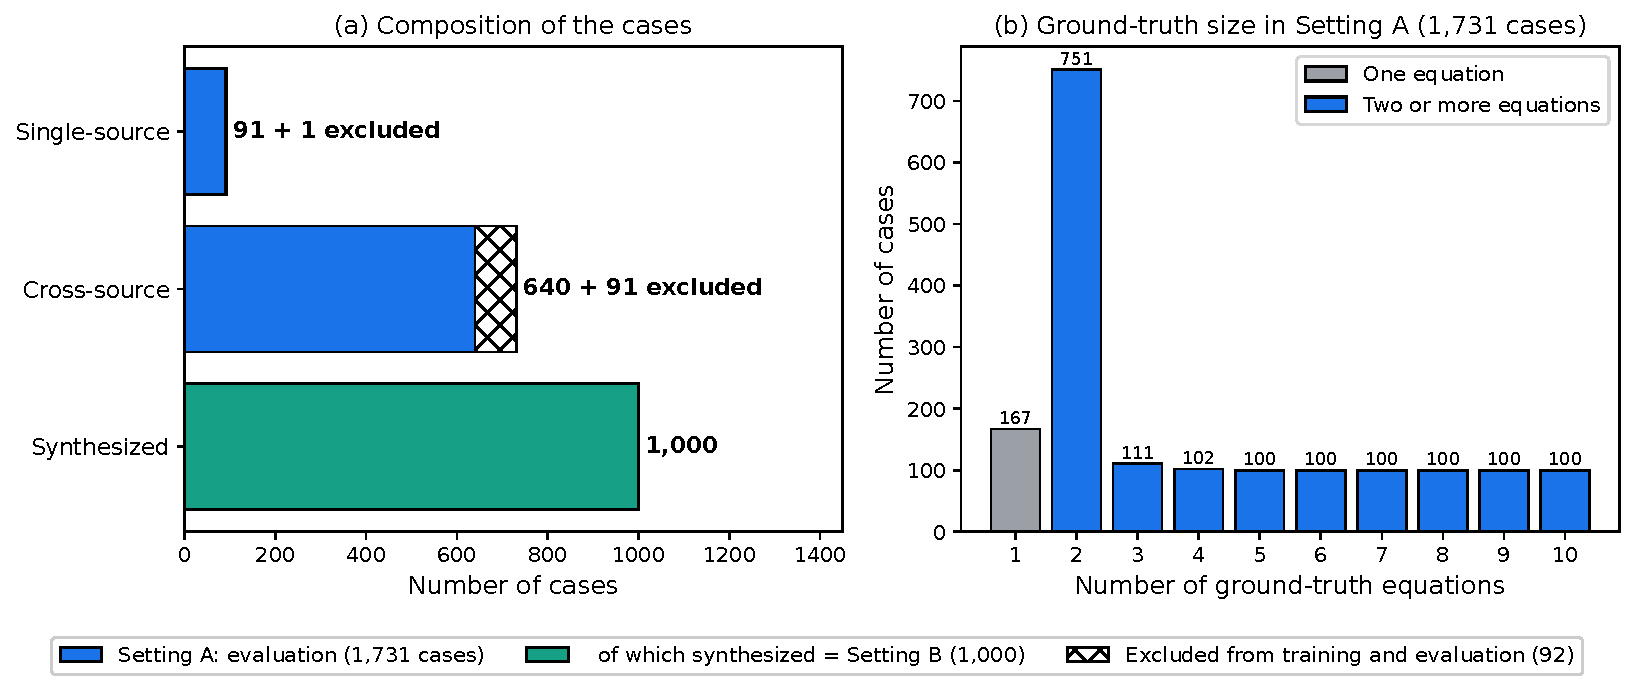
\includegraphics[width=0.98\linewidth]{figures/fig_dataset.pdf}
\caption{The evaluation cases. (a) Composition: Setting~A uses the single-source, cross-source, and
synthesized cases, and Setting~B the synthesized cases alone; hatched bars mark the cases excluded
from training and evaluation. (b) Number of ground-truth equations per case in Setting~A.}
\label{fig:dataset}
\end{figure}

A language model formed the ground truths of the single-source family (\NSingle{} cases). We gave
Gemini 2.5 Pro a catalog of the database as it then stood, which listed for each equation only
its domain label, its variable symbols, and its identifier, which names its source, and asked for
physically meaningful cases: a description, input and output
variables, and a ground-truth set that the inputs determine and that is sufficient and minimal
(\ref{app:prompts}). We kept the cases whose ground-truth equations all exist in the database, whose
input and output variables all appear in them, and whose ground truth has as many unknowns as
equations once the inputs are given. Each ground truth draws on one source. It is the set that the
model judged minimal, not a model that a source presents; \NSingleOneEq{} of the \NSingle{} ground
truths hold a single equation, and \NSingleRefOnly{} draw only on the generated equation sets.

The cross-source family (\NCross{} cases) combines two or three equations from different sources. A
program built \NCrossProgram{} of these cases. It grouped the domain labels into ten categories,
such as reactor, heat transfer, and control, by hand-written word lists; took pairs of categories
that chemical engineering often combines; collected pairs of equations that come from different
sources and share at least two variable symbols; and formed cases whose outputs are one variable
unique to each equation and whose inputs are all other variables. It wrote each description from an
English template. The other cases are \NCrossPicked{} combinations that a coding-assistant language
model (Claude) wrote as physically meaningful and \NCrossReselected{} variants of them with
reselected input and output variables. Claude Opus 4.8 \citep{ClaudeOpus48} rewrote the descriptions
of these variants, and of two of the original combinations, to match their output variables.

A program formed the ground truths of the synthesized family (\NSynth{} cases,
\secref{sec:synth}).

All ground truths meet requirements~1--3 of \secref{sec:formulation}. Because these
requirements only count variables and equations, we also checked that each unknown can be assigned
to an equation of its own. This check, too, only counts: whether the equations then determine the
outputs was judged on a sample alone (\secref{sec:limitations}). We excluded \NExcluded{} generated cases from both training and
evaluation: \NExcludedCross{} cross-source cases in which one ground-truth equation contains input
variables only, so that some unknowns stay undetermined once the inputs are given, and one
single-source case whose ground truth draws on two sources. Requirement~3 holds trivially in
\NReqThreeTrivial{} of the \NCases{} cases, which contain no variable other than the inputs and
outputs, and requirement~4 cannot be checked, because the database does not mark which variables are
constants. Over all cases, \ShareKTwoPlus\% have two or more ground-truth equations, and the mean is
\MeanKAll.

\subsection{Synthesized cases}\label{sec:synth}

The ground truths of the first two families hold at most \MaxKSingle{} equations, so a program
generated larger ones that mix differential and algebraic equations. It fixes a target size $X$ and
works in two phases. First, it picks a differential equation of the database at
random and takes one of its differentiated variables as an output. It then repeatedly adds an
equation that contains a variable, other than that output, of the equations collected so far,
choosing at random among the equations of the first equation's source when any qualifies and among
those of other sources otherwise, until the set holds $X$ equations. Second, it goes through the
added equations, chooses at random one variable of each that is not yet an output, and adds it to
the outputs; every variable left over becomes an input. The resulting sets have as many unknowns as
equations once the inputs are given, and each equation contributes an output of its own, so every
unknown can be matched to its own equation. We generated 100 cases for each $X$ from 1 to 10;
\NSynthOneSource{} of the \NSynth{} cases draw on a single source. A language model, Claude Sonnet
4.5 \citep{ClaudeSonnet45}, wrote only the description of each case; the equation set, the inputs,
and the outputs all follow from the program (\ref{app:example} shows one case).

\subsection{Stratified split by source}\label{sec:split}

We split the cases into training, validation, and test cases by source. We assign each case to the
source that contributes most of its ground-truth equations, and each source goes wholly, with the
cases assigned to it, to one part: 20\% of the sources to testing, 20\% to validation, and 60\% to
training. Two cases assigned to the same source therefore never fall into different parts. A ground
truth that draws on several sources, however, can share equations with the cases of another part.
In Setting~A, \ShareSharedEqA\% of the test cases of the 10 splits share at least one ground-truth
equation with a training case (\ShareSharedEqAMin\% to \ShareSharedEqAMax\% per split): \ShareSharedEqCross\%
of the cross-source, \ShareSharedEqSynth\% of the synthesized, and \ShareSharedEqSingle\% of the
single-source test cases. In Setting~B, \ShareSharedEqB\% do. The reranker reads ten features of a
candidate, not its identity, so it cannot memorize an equation; the test cases are nevertheless not
all new to it at the level of equations. \ref{app:overlap} therefore scores the methods separately
on the test cases that share a ground-truth equation with a training case and on those that share
none. Because sources hold different numbers of cases, the numbers of cases
vary from split to split: \NTestAMin{} to \NTestAMax{} test cases and \NValAMin{} to \NValAMax{}
validation cases in Setting~A.

A random assignment of sources can put the cases with many equations on one side, so we stratify
it. For one split, we draw \NSplitCandidates{} random assignments and take four quantities per
case: the numbers of ground-truth equations, of input variables, of output variables, and of
sources spanned. For each quantity we compute the $L_1$ distance between its training and test
frequency distributions, and we select the assignment with the smallest sum of the four distances
(\ref{app:split} shows one split).
Every experiment repeats this procedure over the same 10 random seeds and reports the mean and the
standard deviation across them; the seed also fixes the initialization of the model and the choice
of incorrect candidates. The validation cases choose the hyperparameters of the methods
(\secref{sec:compared}).

\section{Experimental setup}\label{sec:setup}

\subsection{Settings}\label{sec:settings}

We evaluate the methods in two settings. Setting~A holds all \NCases{} evaluation cases of the three
families, and Setting~B the \NSynth{} synthesized cases alone, 100 for each number of ground-truth
equations from 1 to 10. Every result uses the stratified source-disjoint split of
Section~\ref{sec:split} with the same 10 random seeds.

\subsection{Compared methods}\label{sec:compared}

We compare the proposed method with a classical information-retrieval baseline, two variants of the
baseline with stronger text scorers, and two LLMs. Table~\ref{tab:inputs} lists the information each
method uses.

\begin{table}[tbp]
\centering
\caption{Information used by each method. The baseline includes its variants with BM25 and E5.}
\label{tab:inputs}
\footnotesize
\setlength{\tabcolsep}{4pt}
\begin{tabular}{p{0.44\linewidth}ccc}
\toprule
Information & Proposed & Baseline & LLMs \\
\midrule
Query (description, input and output variables) & yes & yes & yes \\
Expression and domain label of each equation & yes & yes & yes \\
Variable symbols of each equation, as a list & yes & yes & no \\
Context text of each equation & yes & yes & no \\
Source of each equation & no & no & no \\
Cases with known ground truth & training, validation & validation & none \\
\bottomrule
\end{tabular}
\end{table}

\paragraph{Classical baseline} The baseline ranks the whole database by the Stage-1 score of
Eq.~\eqref{eq:stage1}, without a learned model and without a candidate set. Its weights decide how
well it ranks, so we compare \NBasePairs{} weight pairs $(w_{\mathrm{t}}, w_{\mathrm{v}})$ from
$\BasePairFirst$ to $\BasePairLast$ and, in each split, evaluate on the test cases the pair with the highest Recall@20 on
the validation cases (\ref{app:weights}). Two variants test whether stronger text evidence alone
would close the gap to the proposed method. The first replaces the TF-IDF cosine with BM25
\citep{BM25}; the second replaces it with the cosine between dense embeddings of the description
and of each equation text from the sentence encoder E5 \citep{E5}. Both rescale the text score to
$[0, 1]$ over the database for every query, choose their weights on the validation cases in the
same way, and train nothing.

\paragraph{LLMs} An LLM receives the whole database and the query of one test case and returns the
identifiers of 20 equations for the desired model, from the most to the least likely. It sees no
solved case (zero-shot). Each equation reaches it only as its identifier, its expression, and its
domain label: the prompt with the database holds \NDbTokens{} tokens, and adding the variable
definitions and the context texts would exceed the input limit of one million tokens. We withhold
the sources, shuffle the order of the equations, and renumber their identifiers, because the
proposed method does not read the sources and the synthesized ground truths prefer equations of one
source, so the sources would give the LLMs alone a clue to the answer. The prompt states the first
three requirements of Section~\ref{sec:formulation} (\ref{app:prompts}). The models are Claude
Opus~5.5 and Claude Haiku~5.5 \citep{ClaudeModels}, a large and a small model of one vendor, both
with the reasoning effort set to high. An LLM sees no training case, so its input for a case does
not depend on the split; we therefore ask it three times per case, independently, and use the mean
of the three answers in every split in which the case is a test case. The splits of the two
settings hold \NTestDistinct{} distinct test cases, so each model answered \NCalls{} calls.

\paragraph{Proposed method} We compared four pairs of first-stage weights, \StagePairs, by the
Recall@20 of the validation cases. Their validation
Recall@20 ranged only from \ValRecAMin{} to \ValRecAMax{} in Setting~A and from \ValRecBMin{} to
\ValRecBMax{} in Setting~B, so we use the pair $(\WText, \WVar)$ in every split, whose candidate set
admits every ground-truth equation with the smallest $N_1$. In each split we set $N_1$ to the
smallest number of candidates that holds every ground-truth equation of the training and validation
cases, rounded up to the next thousand; this gives $N_1 = \NOne$ in all 10 splits, whereas the
other pairs need \NOneOtherMin{} to \NOneOtherMax. Between random and hard negatives, each split
takes the one with the higher validation Recall@20, and hard negatives won in all \NSplitsAll{}
splits of the two settings. The other hyperparameters are a reference set of $m = \RefSize$
equations, the margin $\gamma = \Margin$, $n_{\mathrm{neg}} = \NNeg$ incorrect candidates, and
\Epochs{} epochs of AdamW with learning rate $\LearnRate$; we have not compared them with other
values.

\subsection{Judgment and metrics}\label{sec:metrics}

Every method returns identifiers of database equations: the retrieval methods rank the database,
and the LLMs list identifiers. A returned equation is correct when its identifier belongs to the
ground truth $\mathcal{R}_q$; an identifier absent from the database counts as incorrect and keeps
its rank, and a repeated identifier counts only at its first occurrence. For each test case we
compute the following quantities and average them over the test cases of a split;
$\Top_n(q)$ denotes the top $n$ equations that a method returns.
\begin{itemize}
  \item Recall@20 $= |\mathcal{R}_q \cap \Top_{20}(q)| / K$, the primary metric: the fraction of
    the ground-truth equations among the 20 equations presented.
  \item Mean average precision (MAP): the mean over cases of the average precision
    $\mathrm{AP}(q) = \frac{1}{K} \sum_{e \in \mathcal{R}_q} P(e)$, where $P(e)$ is the fraction of
    ground-truth equations among the equations ranked at or above $e$, and $P(e) = 0$ when $e$ is
    not in the ranking. MAP shows how closely the ground-truth equations crowd at the top. Because
    an LLM returns only 20 equations, the comparison with LLMs uses MAP@20, in which $P(e) = 0$ for
    every ground-truth equation outside the top 20.
  \item R-Precision $= |\mathcal{R}_q \cap \Top_K(q)| / K$: the fraction of the ground-truth
    equations within the top $K$ \citep{Manning}.
\end{itemize}
We run no statistical tests. To compare two methods, we report the mean of their difference over
the 10 splits and the number of splits in which one beats the other.

\subsection{Implementation}\label{sec:impl}

Every experiment runs as a deterministic script: the random seed fixes the split, the model
initialization, and the choice of incorrect candidates. The proposed method calls no language model
at inference. One run of training and evaluation for a split of Setting~A took \TimeRunA{} seconds on
average, with six runs in parallel on the CPU of a laptop computer (\ref{app:n1}).

\section{Results}\label{sec:results}

\subsection{Overall comparison}\label{sec:overall}

Table~\ref{tab:overall} and Fig.~\ref{fig:comparison} compare the proposed method with the
classical baseline. With $N_1 = \NOne$, the first stage admitted every ground-truth equation of
every test case in all 10 splits. The proposed method beat the baseline on every metric, in both
settings, and in all 10 splits. Static reranking raised Recall@20 from \RecABase{} to \RecAProp{}
($\DiffRecAPropBase$) and MAP from \MapABase{} to \MapAProp{} ($\DiffMapAPropBase$) in Setting~A,
and Recall@20 from \RecBBase{} to \RecBProp{} ($\DiffRecBPropBase$) and MAP from \MapBBase{} to
\MapBProp{} ($\DiffMapBPropBase$) in Setting~B. Learned greedy selection raised MAP further, to
\MapAGreedy{} and \MapBGreedy{} (Section~\ref{sec:greedyresults}). The variants of the baseline
with BM25 and E5 ranked no better than the TF-IDF baseline --- Recall@20 of \RecABm{} and
\RecAEFive{} in Setting~A and \RecBBm{} and \RecBEFive{} in Setting~B --- and the proposed method
beat them, too, on every metric in all 10 splits (\ref{app:weights}).

\begin{table}[tbp]\centering
\caption{Overall comparison (mean $\pm$ SD over 10 stratified splits). The baseline ranks the whole
database by the weighted sum of the TF-IDF text similarity and the variable overlap, with the
weights chosen on the validation cases of each split.}
\label{tab:overall}
\footnotesize
\setlength{\tabcolsep}{4pt}
\begin{tabular}{llccc}
\toprule
Setting & Method & Recall@20 & MAP & R-Precision \\
\midrule
A & Baseline & $\RecABase \pm \RecABaseSD$ & $\MapABase \pm \MapABaseSD$ & $\RPrecABase \pm \RPrecABaseSD$ \\
 & Proposed, static reranking & $\RecAProp \pm \RecAPropSD$ & $\MapAProp \pm \MapAPropSD$ & $\RPrecAProp \pm \RPrecAPropSD$ \\
 & Proposed, learned greedy & $\RecAGreedy \pm \RecAGreedySD$ & $\MapAGreedy \pm \MapAGreedySD$ & $\RPrecAGreedy \pm \RPrecAGreedySD$ \\
\midrule
B & Baseline & $\RecBBase \pm \RecBBaseSD$ & $\MapBBase \pm \MapBBaseSD$ & $\RPrecBBase \pm \RPrecBBaseSD$ \\
 & Proposed, static reranking & $\RecBProp \pm \RecBPropSD$ & $\MapBProp \pm \MapBPropSD$ & $\RPrecBProp \pm \RPrecBPropSD$ \\
 & Proposed, learned greedy & $\RecBGreedy \pm \RecBGreedySD$ & $\MapBGreedy \pm \MapBGreedySD$ & $\RPrecBGreedy \pm \RPrecBGreedySD$ \\
\bottomrule
\end{tabular}
\end{table}

\begin{figure}[tbp]\centering
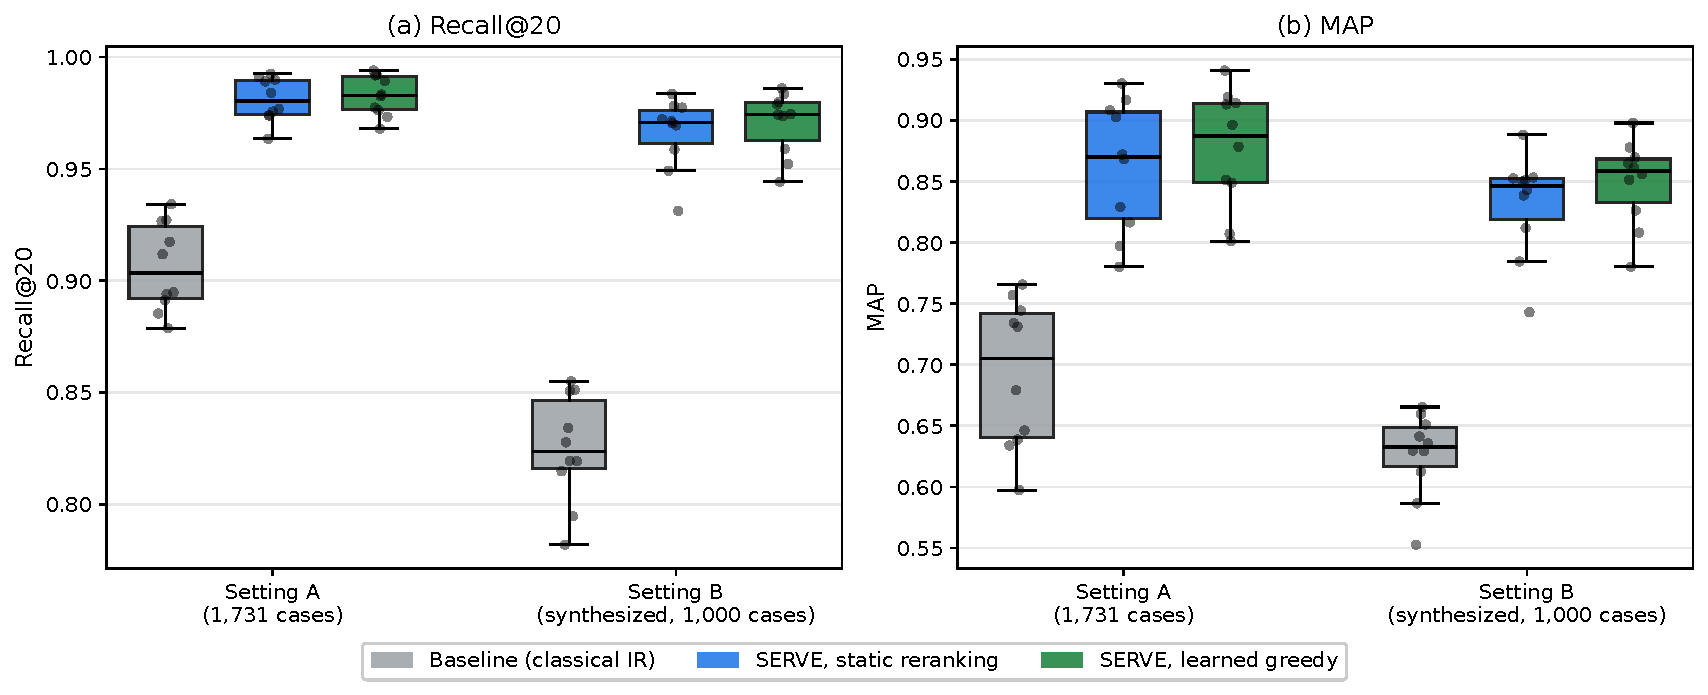
\includegraphics[width=\linewidth]{figures/fig_method_comparison.pdf}
\caption{(a) Recall@20 and (b) MAP of the classical baseline and of the proposed method with static
reranking and with learned greedy selection in Settings~A and~B. Boxes show the 10 stratified
splits, and dots the individual splits.}
\label{fig:comparison}
\end{figure}

\subsection{Comparison with LLMs}\label{sec:llmresults}

Table~\ref{tab:llm} compares static reranking and the baseline with the two LLMs. In Setting~A,
Recall@20 reached \RecAProp{} for the proposed method, \RecAOpus{} for Claude Opus~5.5, and
\RecAHaiku{} for Claude Haiku~5.5. The proposed method beat both LLMs in Recall@20 and in MAP@20 in
all 10 splits of both settings; its lead over Opus~5.5 in Setting~A averaged \GapRecAOpusProp{} in
Recall@20 and \GapMapTwAOpusProp{} in MAP@20. Opus~5.5 beat the baseline in both metrics in all 10
splits of both settings, by \GapRecAOpusBase{} in Recall@20 and \GapMapTwAOpusBase{} in MAP@20 in
Setting~A and by \GapRecBOpusBase{} and \GapMapTwBOpusBase{} in Setting~B. Haiku~5.5 fell below the
baseline in both metrics in all 10 splits.

\begin{table}[tbp]\centering
\caption{Comparison with LLMs (mean $\pm$ SD over 10 stratified splits). The LLMs answered each case
three times; a case takes the mean of its three answers.}
\label{tab:llm}
\footnotesize
\setlength{\tabcolsep}{4pt}
\begin{tabular}{lcccc}
\toprule
 & \multicolumn{2}{c}{Setting A} & \multicolumn{2}{c}{Setting B} \\
\cmidrule(lr){2-3}\cmidrule(l){4-5}
Method & Recall@20 & MAP@20 & Recall@20 & MAP@20 \\
\midrule
Baseline & $\RecABase \pm \RecABaseSD$ & $\MapTwABase \pm \MapTwABaseSD$ & $\RecBBase \pm \RecBBaseSD$ & $\MapTwBBase \pm \MapTwBBaseSD$ \\
Proposed, static reranking & $\RecAProp \pm \RecAPropSD$ & $\MapTwAProp \pm \MapTwAPropSD$ & $\RecBProp \pm \RecBPropSD$ & $\MapTwBProp \pm \MapTwBPropSD$ \\
Claude Opus 5.5 & $\RecAOpus \pm \RecAOpusSD$ & $\MapTwAOpus \pm \MapTwAOpusSD$ & $\RecBOpus \pm \RecBOpusSD$ & $\MapTwBOpus \pm \MapTwBOpusSD$ \\
Claude Haiku 5.5 & $\RecAHaiku \pm \RecAHaikuSD$ & $\MapTwAHaiku \pm \MapTwAHaikuSD$ & $\RecBHaiku \pm \RecBHaikuSD$ & $\MapTwBHaiku \pm \MapTwBHaikuSD$ \\
\bottomrule
\end{tabular}
\end{table}

Table~\ref{tab:llmkind} breaks Setting~A down by family; a split holds \NTestSingleMin{} to
\NTestSingleMax{} single-source, \NTestCrossMin{} to \NTestCrossMax{} cross-source, and
\NTestSynthMin{} to \NTestSynthMax{} synthesized test cases. In every family, Opus~5.5 was below
the proposed method. The gap was smallest on the single-source cases (\LeadRecSingle{} in
Recall@20 and \LeadMapTwSingle{} in MAP@20) and larger on the cross-source cases (\LeadRecCross{}
and \LeadMapTwCross) and the synthesized cases (\LeadRecSynth{} and \LeadMapTwSynth). Against the
baseline, Opus~5.5 was higher in both metrics
on the synthesized cases, lower in both on the single-source cases, and higher in MAP@20 but lower
in Recall@20 on the cross-source cases. Haiku~5.5 was below the baseline in every family; its
Recall@20 on the cross-source cases was \RecCrossHaiku.

\begin{table}[tbp]\centering
\caption{Comparison with LLMs by family in Setting~A (mean $\pm$ SD over 10 stratified splits).}
\label{tab:llmkind}
\scriptsize
\setlength{\tabcolsep}{2.5pt}
\begin{tabular}{lcccccc}
\toprule
 & \multicolumn{2}{c}{Single-source} & \multicolumn{2}{c}{Cross-source} & \multicolumn{2}{c}{Synthesized} \\
\cmidrule(lr){2-3}\cmidrule(lr){4-5}\cmidrule(l){6-7}
Method & Recall@20 & MAP@20 & Recall@20 & MAP@20 & Recall@20 & MAP@20 \\
\midrule
Baseline & $\RecSingleBase \pm \RecSingleBaseSD$ & $\MapTwSingleBase \pm \MapTwSingleBaseSD$ & $\RecCrossBase \pm \RecCrossBaseSD$ & $\MapTwCrossBase \pm \MapTwCrossBaseSD$ & $\RecSynthBase \pm \RecSynthBaseSD$ & $\MapTwSynthBase \pm \MapTwSynthBaseSD$ \\
Proposed & $\RecSingleProp \pm \RecSinglePropSD$ & $\MapTwSingleProp \pm \MapTwSinglePropSD$ & $\RecCrossProp \pm \RecCrossPropSD$ & $\MapTwCrossProp \pm \MapTwCrossPropSD$ & $\RecSynthProp \pm \RecSynthPropSD$ & $\MapTwSynthProp \pm \MapTwSynthPropSD$ \\
Opus 5.5 & $\RecSingleOpus \pm \RecSingleOpusSD$ & $\MapTwSingleOpus \pm \MapTwSingleOpusSD$ & $\RecCrossOpus \pm \RecCrossOpusSD$ & $\MapTwCrossOpus \pm \MapTwCrossOpusSD$ & $\RecSynthOpus \pm \RecSynthOpusSD$ & $\MapTwSynthOpus \pm \MapTwSynthOpusSD$ \\
Haiku 5.5 & $\RecSingleHaiku \pm \RecSingleHaikuSD$ & $\MapTwSingleHaiku \pm \MapTwSingleHaikuSD$ & $\RecCrossHaiku \pm \RecCrossHaikuSD$ & $\MapTwCrossHaiku \pm \MapTwCrossHaikuSD$ & $\RecSynthHaiku \pm \RecSynthHaikuSD$ & $\MapTwSynthHaiku \pm \MapTwSynthHaikuSD$ \\
\bottomrule
\end{tabular}
\end{table}

The answers of an LLM vary from run to run. Over the three runs of a case, the standard deviation
of Recall@20 averaged \RunSdOpus{} for Opus~5.5 and \RunSdHaiku{} for Haiku~5.5, and the three runs
gave the same Recall@20 in \RunSameOpus\% and \RunSameHaiku\% of the cases. The sets of identifiers
agreed less than the scores: the Jaccard similarity between two runs averaged \JaccardOpus{} and
\JaccardHaiku, and all three runs returned the same list in \SameListOpus\% and \SameListHaiku\% of
the cases.

The answers did not always take the form that the instruction asked for: 20 identifiers, each
listed once and all taken from the database. Opus~5.5 answered every call and followed the
instruction in \OpusAsInstructed{} of its \NCalls{} answers (\ShareOpusAsInstructed\%);
\OpusUnderTwenty{} answers listed fewer than 20 distinct identifiers, \OpusOverTwenty{} listed
more, \OpusRepeatedId{} repeated an identifier, and \OpusInvalidId{} contained an identifier absent
from the database. For Haiku~5.5, the safety filter of the service stopped \HaikuRefusals{} calls
(\ShareHaikuRefusals\%), which we scored as answers with no correct equation;
\HaikuAsInstructed{} answers (\ShareHaikuAsInstructed\%) followed the instruction,
\HaikuOverTwenty{} listed more than 20 distinct identifiers, \HaikuUnderTwenty{} listed fewer, and
\HaikuRepeatedId{} repeated an identifier.

The \NCalls{} calls cost \CostOpus{} US dollars for Opus~5.5 and \CostHaiku{} for Haiku~5.5,
\CostTotal{} in all, at the prices of November 2026 \citep{AnthropicPricing}. Reading the cached
database at every call made up \ReadShareOpus\% and \ReadShareHaiku\% of these amounts.

\subsection{Performance by case characteristics}\label{sec:bycharacteristics}

Fig.~\ref{fig:characteristic} breaks the comparison with the baseline down by the number of
ground-truth equations and by the number of input variables in Setting~A, pooling the test cases of
the 10 splits: \NRecordsA{} records of \NDistinctA{} distinct cases. On the cases with one
ground-truth equation, both methods reach a Recall@20 of \RecKOneProp, and their MAP is nearly the same:
\MapKOneProp{} for static reranking and \MapKOneBase{} for the baseline. From two equations on, the
gap grows with the number of equations: Recall@20 differs by $\DiffRecKTwo$ at two equations,
$\DiffRecKFive$ at five, and $\DiffRecKTen$ at ten. By the number of input variables, the gap in
Recall@20 grows from $\DiffRecInLow$ at five or fewer to $\DiffRecInHigh$ at 21 or more. The
classical baseline finds a single equation as well as the proposed method does, and the lead
of the proposed method grows with the numbers of ground-truth equations and input variables.

\begin{figure}[tbp]\centering
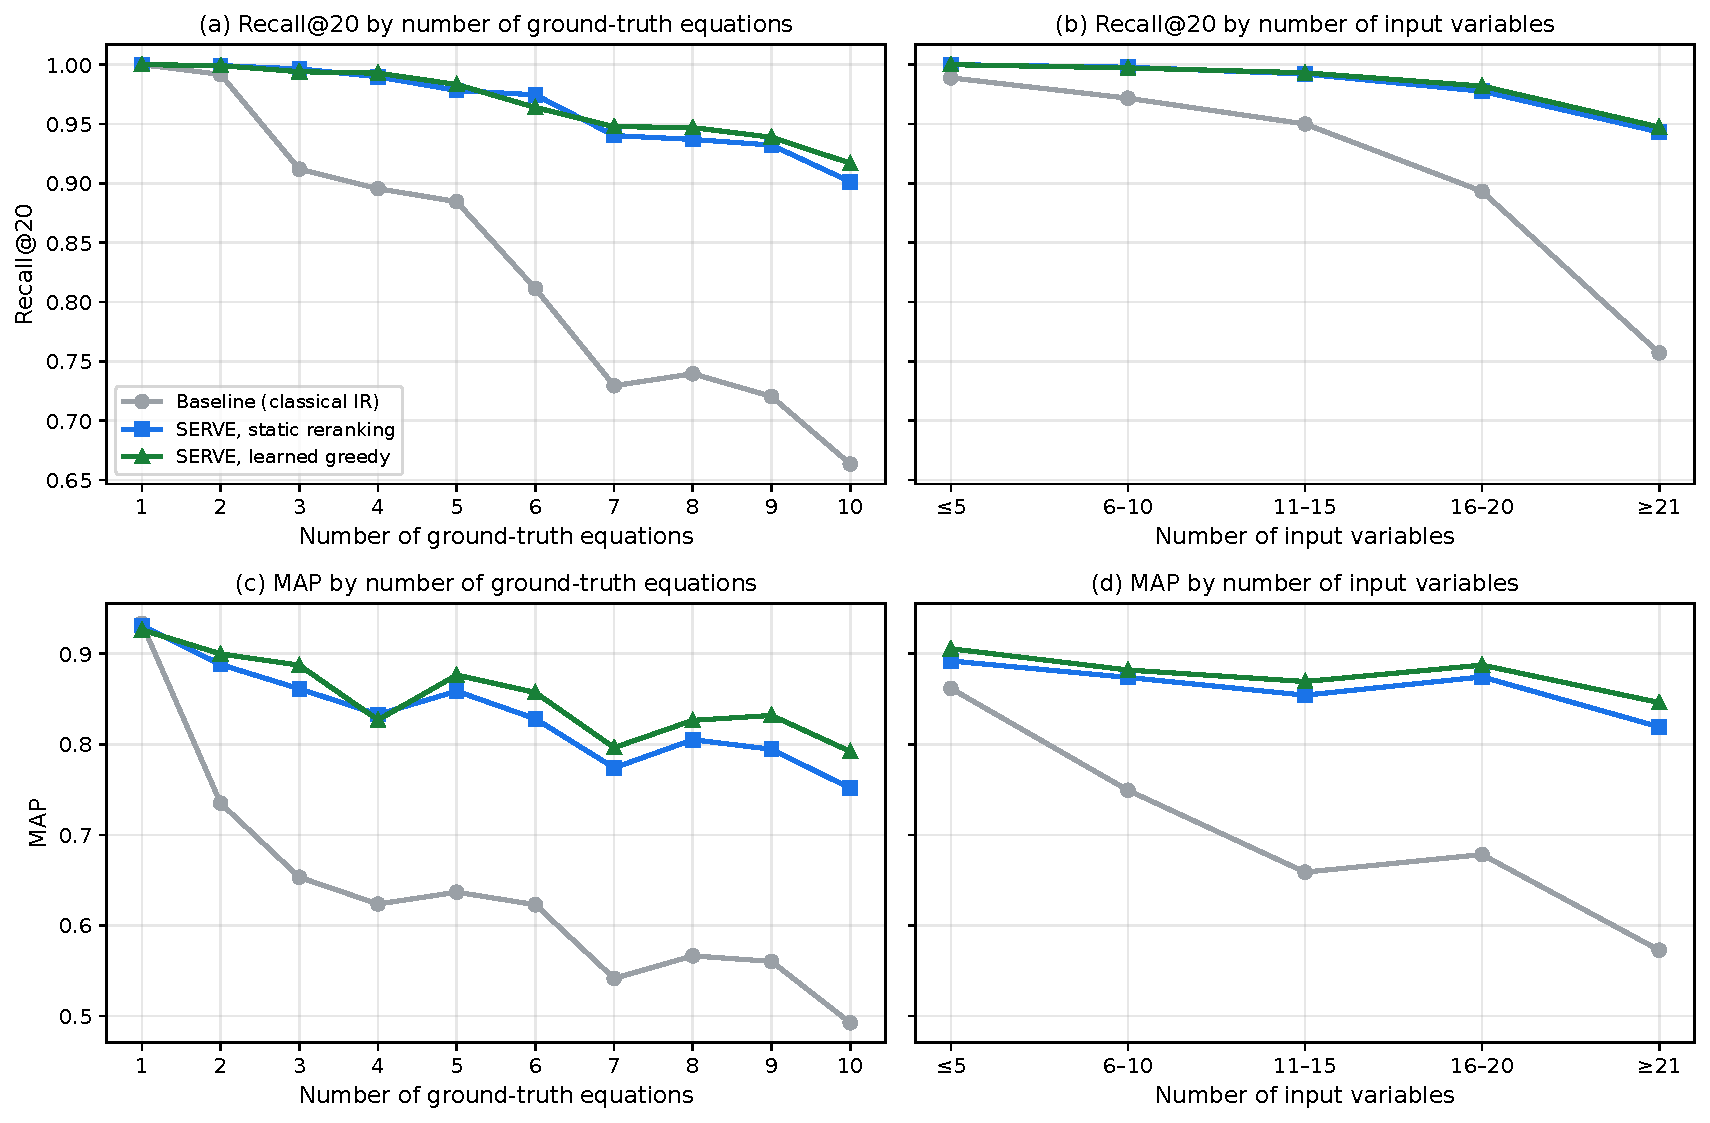
\includegraphics[width=\linewidth]{figures/fig_characteristic.pdf}
\caption{Recall@20 (a, b) and MAP (c, d) in Setting~A by the number of ground-truth equations
(a, c) and by the number of input variables (b, d). Each point pools the test cases of the 10
splits and carries no error bar; Fig.~\ref{fig:comparison} shows the spread across splits of the
overall values.}
\label{fig:characteristic}
\end{figure}

\subsection{Sources of the improvement}\label{sec:mechanism}

We decompose the gain of static reranking over the baseline with the same weights
$(\WText, \WVar)$ --- $\DiffRecATotal$ in Recall@20 and $\DiffMapATotal$ in MAP in Setting~A --- by
growing the feature set of the reranker, retraining it at every step, and evaluating it on the same
10 splits.
\begin{enumerate}
  \item Learning the weights: a reranker that reads only the two Stage-1 terms, $f_1$ and $f_2$,
    moves Recall@20 from \RecASameW{} to \RecARTwo{} and MAP from \MapASameW{} to \MapARTwo, and
    beats the baseline in only \WinsRecStepOne{} of the 10 splits in Recall@20 and \WinsMapStepOne{} in
    MAP. Relearning how to weight the two terms does not raise the accuracy.
  \item Per-equation features: adding the other five query--equation features raises Recall@20 to
    \RecARSeven{} ($\DiffRecStepTwo$) and MAP to \MapARSeven{} ($\DiffMapStepTwo$), in all 10
    splits. Specificity $f_6$ alone carries nearly all of this step: adding it alone reaches a
    Recall@20 of \RecASpec{} ($\DiffRecSpec$) and a MAP of \MapASpec{} ($\DiffMapSpec$). The
    benchmark makes this feature decisive: in \NReqThreeTrivial{} of the \NCases{} cases the query
    lists every variable of the ground truth (Section~\ref{sec:cases}), so every ground-truth
    equation has a specificity of one.
  \item Set-aware features: adding the three of them raises Recall@20 to \RecAProp{}
    ($\DiffRecStepThree$, in \WinsRecStepThree{} of the 10 splits) and MAP to \MapAProp{}
    ($\DiffMapStepThree$, in all \WinsMapStepThree). Recall@20 leaves little room at \RecARSeven, so the set-aware
    features mainly raise the ground-truth equations within the top 20.
\end{enumerate}
Added one at a time to the seven features, complementarity raises MAP by $\DiffMapComp$ and
coherence by $\DiffMapCoh$, each in all 10 splits, and domain agreement by $\DiffMapDomAgree$, in
\WinsMapDomAgree{} of the 10. All three together add about what complementarity or coherence adds
alone, so the effects of these two overlap. The MAP gain of the set-aware features is
$\LiftMapKOne$ on the cases with one ground-truth equation, which give a candidate no other equation
to relate to, and $\LiftMapKMin$ to $\LiftMapKMax$ at every larger number of equations, in all 10
splits (\ref{app:bucket}).

Permutation feature importance measures, without retraining, how much the trained model relies on
each feature. We fixed the trained ten-feature model, shuffled the values of one feature among the
candidates of each test case, and measured Recall@20 and MAP, averaging over \NPerm{} shuffles
(Fig.~\ref{fig:pfi}). Shuffling the six variable-overlap features ($f_2$, $f_4$--$f_6$,
$g_{\mathrm{Comp}}$, $g_{\mathrm{Coh}}$) together lowers Recall@20 from \RecAProp{} to \PfiRecVar{}
and MAP from \MapAProp{} to \PfiMapVar, in all 10 splits. Among single features, specificity matters
most: shuffling it alone lowers Recall@20 to \PfiRecSpec. Shuffling the four topic features ($f_1$,
$f_3$, $f_7$, $g_{\mathrm{Dom}}$) together leaves Recall@20 at \PfiRecTopic{} and MAP at
\PfiMapTopic; the drops, \PfiDropRecTopic{} and \PfiDropMapTopic, are small but appear in all 10
splits. Ablation asks what a feature adds when the model is retrained with it, and permutation
importance asks how much a fixed model relies on it; both reach the same conclusion: the features
that read variable overlap decide most of the accuracy.

\begin{figure}[tbp]\centering
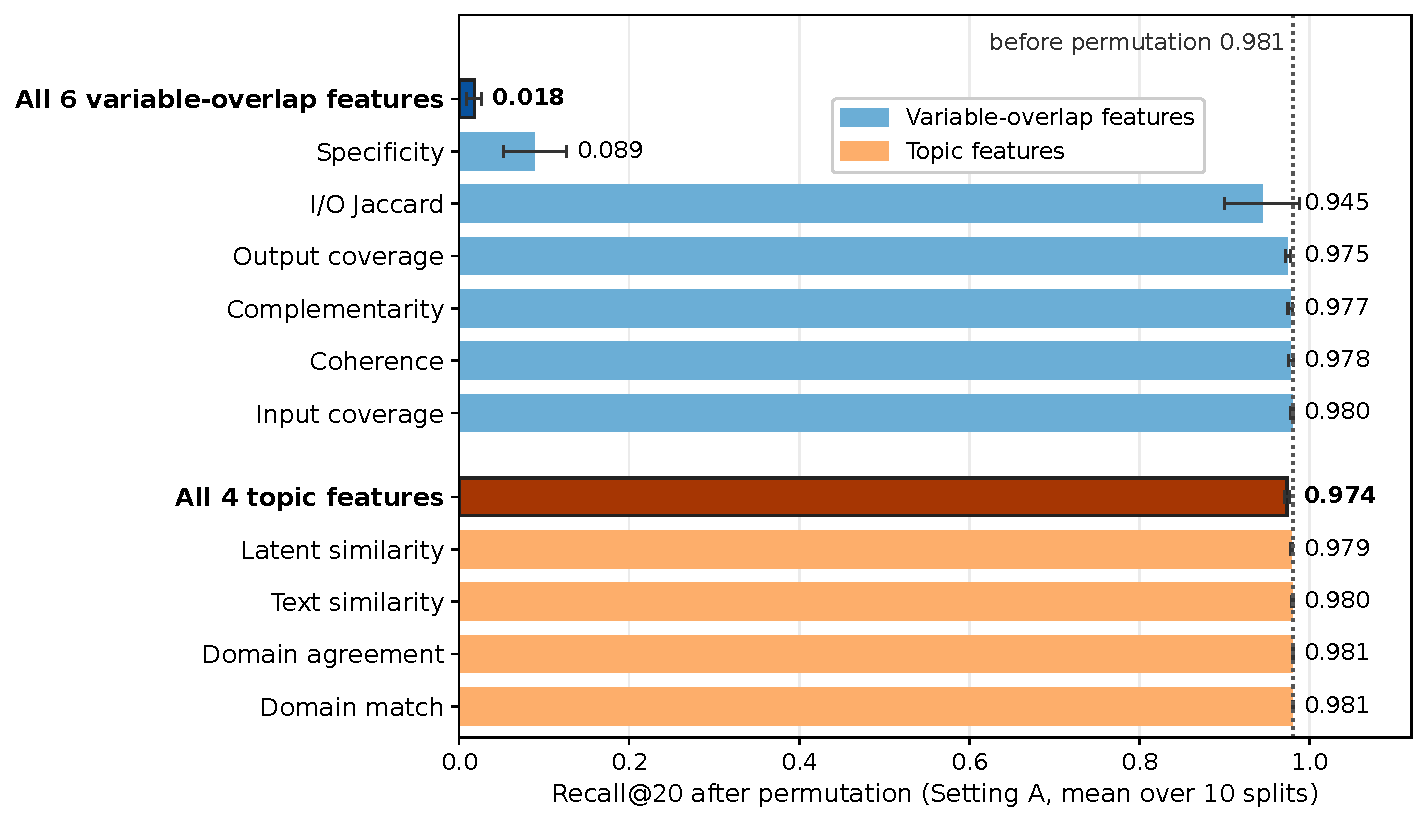
\includegraphics[width=0.78\linewidth]{figures/fig_pfi.pdf}
\caption{Recall@20 after the values of a feature are shuffled among the candidates of each case
(Setting~A, static reranking). Bars show the mean over the 10 splits, error bars the SD of the drop
across the splits, and the dotted line the Recall@20 before the shuffle. The first, darker bar of
each group shuffles all its features together.}
\label{fig:pfi}
\end{figure}

\subsection{Sequential selection}\label{sec:greedyresults}

We compared static reranking, greedy selection at inference, and learned greedy selection
(Section~\ref{sec:seq}) on the same 10 splits (Table~\ref{tab:greedy}; \ref{app:bucket} shows the
spread across the splits). Recall@20 hardly differs
among the three, because the top 20 already hold nearly every ground-truth equation; the strategies
differ in how they order the equations within the top 20. Greedy selection at inference beats
static reranking in MAP by $\DiffMapAInferProp$ in Setting~A and $\DiffMapBInferProp$ in Setting~B,
in all 10 splits of each. Learned greedy selection adds little to it: $\DiffMapAGreedyInfer$ in
Setting~A (\WinsMapAGreedyInfer{} of the 10 splits) and $\DiffMapBGreedyInfer$ in Setting~B
(\WinsMapBGreedyInfer{} of the 10). The differences grow on the cases with eight or more
ground-truth equations, \NRecEightA{} test records in Setting~A and \NRecEightB{} in Setting~B over
the 10 splits. On these cases, learned greedy selection beats static reranking in MAP by
$\DiffMapAEight$ and $\DiffMapBEight$ and in R-Precision by $\DiffRPrecAEight$ and
$\DiffRPrecBEight$ (all 10 splits), and in Recall@20 by $\DiffRecAEight$ and $\DiffRecBEight$
(\WinsRecAEight{} and \WinsRecBEight{} of the 10 splits). Sequential selection thus pays off on the
cases with many ground-truth equations, the cases that motivated it.

\begin{table}[tbp]\centering
\caption{The three selection strategies (mean over 10 splits). The rows ``eight or more'' average
only the cases with eight or more ground-truth equations.}
\label{tab:greedy}
\small
\setlength{\tabcolsep}{4pt}
\begin{tabular}{llccc}
\toprule
 & & Static & Greedy at inference & Learned greedy \\
\midrule
Setting A & Recall@20 & \RecAProp & \RecAInfer & \RecAGreedy \\
 & MAP & \MapAProp & \MapAInfer & \MapAGreedy \\
 & R-Precision & \RPrecAProp & \RPrecAInfer & \RPrecAGreedy \\
 & MAP, eight or more & \MapAEightProp & \MapAEightInfer & \MapAEightGreedy \\
\midrule
Setting B & Recall@20 & \RecBProp & \RecBInfer & \RecBGreedy \\
 & MAP & \MapBProp & \MapBInfer & \MapBGreedy \\
 & R-Precision & \RPrecBProp & \RPrecBInfer & \RPrecBGreedy \\
 & MAP, eight or more & \MapBEightProp & \MapBEightInfer & \MapBEightGreedy \\
\bottomrule
\end{tabular}
\end{table}

\subsection{Topic features}\label{sec:nullresult}

Four of the ten features read topical closeness: the text similarity $f_1$, the latent similarity
$f_3$, the domain match $f_7$, and the domain agreement $g_{\mathrm{Dom}}$. They rest on a
reasonable expectation, that the equations of one model share a topic, yet adding the latter three
one at a time did not raise Recall@20 in Setting~A. Added to the two-feature reranker, the domain match
changed Recall@20 by $\DiffRecDomMatch$ (higher in \WinsRecDomMatch{} of the 10 splits) and the
latent similarity by $\DiffRecLatent$ (\WinsRecLatent{} of 10); added to the seven-feature reranker,
the domain agreement changed Recall@20 by $\DiffRecDomAgree$ (\WinsRecDomAgree{} of 10), although
it raised MAP by $\DiffMapDomAgree$ (Section~\ref{sec:mechanism}). Coarser domain labels did not
help either: after we merged the labels in three ways, by unifying their spelling and by clustering
them into 100 and into 40 groups, adding the domain match changed Recall@20 by $\DiffRecMergeWorst$
to $\DiffRecMergeBest$.

The topic features add little because the variable-overlap features alone nearly separate the
correct candidates from the incorrect ones. We measured how well one feature alone separates them
by the area under the receiver-operating-characteristic curve (AUC): within each case we formed
every pair of a correct and an incorrect equation, took the fraction of pairs in which the correct
equation has the higher value (a tie counting one half), and averaged over the cases, with the
incorrect equations drawn either from the whole database or from the candidates
(Table~\ref{tab:auc}). Within the candidates, the AUC is \AucCandIoJac{} for the I/O Jaccard and
\AucCandSpec{} for specificity, above the \AucCandLatent{} of the latent similarity and the
\AucCandText{} of the text similarity. The topic features do separate the ground-truth equations,
but less sharply than features the model already has.

\begin{table}[tbp]\centering
\caption{How well one feature alone separates the ground-truth equations from the incorrect ones
(AUC; mean $\pm$ standard error over the cases of Setting~A). The columns differ in where the
incorrect equations come from.}
\label{tab:auc}
\small
\begin{tabular}{lcc}
\toprule
Feature & Whole database & Within the candidates \\
\midrule
I/O Jaccard $f_2$ & $\AucFullIoJac \pm \AucFullIoJacSE$ & $\AucCandIoJac \pm \AucCandIoJacSE$ \\
Specificity $f_6$ & $\AucFullSpec \pm \AucFullSpecSE$ & $\AucCandSpec \pm \AucCandSpecSE$ \\
Latent similarity $f_3$ & $\AucFullLatent \pm \AucFullLatentSE$ & $\AucCandLatent \pm \AucCandLatentSE$ \\
Text similarity $f_1$ & $\AucFullText \pm \AucFullTextSE$ & $\AucCandText \pm \AucCandTextSE$ \\
Domain agreement $g_{\mathrm{Dom}}$ & $\AucFullDomAgree \pm \AucFullDomAgreeSE$ & $\AucCandDomAgree \pm \AucCandDomAgreeSE$ \\
Domain match $f_7$ & $\AucFullDomMatch \pm \AucFullDomMatchSE$ & $\AucCandDomMatch \pm \AucCandDomMatchSE$ \\
\bottomrule
\end{tabular}
\end{table}

\subsection{Error analysis}\label{sec:erroranalysis}

\paragraph{Misses of the proposed method} We examined one split, that with seed \FirstSeed: its
\NErrCases{} test cases hold \NErrGt{} ground-truth equations, and its Recall@20 is \ErrRecall.
Static reranking left \NMissed{} of the ground-truth equations out of its top 20. The candidates
contained every ground-truth equation, so the second stage, not the first, missed all of them. The
\NSolved{} cases with every ground-truth equation in the top 20 average \MeanKSolved{} ground-truth
equations and \MeanInSolved{} input variables, against \MeanKUnsolved{} and \MeanInUnsolved{} for
the \NUnsolved{} cases with misses. In each of these cases we paired each missed equation with
each incorrect equation in the top 20 and took the fraction of pairs in which the missed equation
has the higher value of a feature, a tie counting one half. Averaged over the cases, the fraction
is \RescueLatent{} for the latent similarity, \RescueText{} for the text similarity, \RescueSpec{}
for specificity, and \RescueJac{} for the I/O Jaccard. Every fraction lies near or below one half,
so the present features cannot repair these errors. Specificity cannot by construction: where the
query lists every variable of the ground truth, as it does in \NReqThreeTrivial{} of the \NCases{}
cases, every ground-truth equation has a specificity of one, and so has every other equation whose
variables all belong to the query. The features that compare the variables of an equation with
the query ($f_2$, $f_4$, $f_5$, $f_6$) also cannot order two equations that hold the same
variables. For the one-equation case whose ground truth is the linearized balance of the
concentration deviation $C_A'$ of a reactor, the database holds a second equation, the balance of
the temperature deviation $T'$, with the same variable set, and these four features take the same
values for both.

\paragraph{Cases in which the LLM does better} We compared, case by case, the mean Recall@20 of
Opus~5.5 over its three runs with that of static reranking over the splits in which the case is a
test case. Of the \NDistinctA{} distinct test cases of Setting~A, Opus~5.5 was higher in
\NOpusWinRec{} (\ShareOpusWinRec\%), equal in \NOpusTieRec, and lower in \NOpusLossRec; in MAP@20
it was higher in \NOpusWinMap{} and lower in \NOpusLossMap. All \NOpusWinRec{} cases are synthesized
cases, and \NOpusWinSevenPlus{} of them have seven or more ground-truth equations. In
\NOpusWinCopies{} of the \NOpusWinRec{} cases, equations with the same expression as a ground-truth
equation but another identifier appeared in the top 20 of both methods (\CopiesPerListProp{} per
list for static reranking and \CopiesPerListOpus{} for Opus~5.5), and the judgment by identifiers
counts them as incorrect.

The two methods fill the rest of the list differently. On the synthesized cases with seven or more
ground-truth equations in which Opus~5.5 was higher, static reranking placed \WrongInIoProp{}
incorrect equations per list whose variables all belong to the query variables, against
\WrongInIoOpus{} for Opus~5.5. Static reranking placed about as many where Opus~5.5 was equal or
lower (\WrongInIoPropTie{} and \WrongInIoPropLoss), so this is a general habit of the reranker:
specificity, its strongest feature, rewards exactly such equations. In the \NOpusWinRec{} cases in
which Opus~5.5 was higher, it placed \NOnlyOpusEq{} ground-truth equations in the top 20 in at
least two of its three runs that static reranking placed in fewer than half of the splits, and
static reranking placed \NOnlyPropEq{} that Opus~5.5 did not. The \NOnlyOpusEq{} equations overlap
less with the query variables than the \NBothEq{} equations that both methods placed (mean I/O
Jaccard \JacOnlyOpus{} against \JacBoth),
resemble the description less (text similarity \TextOnlyOpus{} against \TextBoth), hold fewer
variables (\VarsOnlyOpus{} against \VarsBoth), and rank lower in the first stage (median rank
\RankOnlyOpus{} against \RankBoth). Examples are the steady-state form of a balance,
$0 = w_1 x_1 + w_2 x_2 - w x$ for a blending tank, and a definition,
$\hat{H} = C (T - T_{\mathrm{ref}})$ for an enthalpy.

The cross-source cases show the same dependence in MAP@20. We sorted them into thirds by the
smallest I/O Jaccard among the ground-truth equations of a case. The MAP@20 of static reranking
falls from \TerHighProp{} and \TerMidProp{} in the upper two thirds to \TerLowProp{} in the lowest,
whereas that of Opus~5.5 stays between \TerOpusMin{} and \TerOpusMax; Opus~5.5 had the higher
MAP@20 in \TerLowWin\% of the cases of the lowest third, against \TerMidWin\% and \TerHighWin\% of
the other two. In the cross-source cases in which Opus~5.5 had the higher MAP@20, its first-ranked
equation was a ground-truth equation in \RankOneCrossOpus\% of its answers, against
\RankOneCrossProp\% of the lists of static reranking.

\section{Discussion}\label{sec:discussion}

\subsection{Strengths and weaknesses of the two approaches}\label{sec:strengths}

The comparison of Section~\ref{sec:llmresults} shows where a retrieval method trained for the task
and an LLM that reads the whole database each do well.

The proposed method is the more accurate of the two, and its lead grows with the size of the model:
it is smallest on the single-source cases and largest on the cross-source and synthesized cases,
whose ground truths combine sources or hold many equations (Table~\ref{tab:llmkind}). The method
reads the variable symbols of every equation and learns from cases with known ground truths how
the variables of a model fit together, so it can collect many equations through the variables they
share. It returns the same ranking for the same query, calls no external service, and trains in
minutes; the size of the database it can search is not bounded by an input limit. Its weaknesses
follow from the same reliance on variable overlap. It needs cases with known ground truths for
training, and it fills the top of the list with equations whose variables all belong to the query,
which pushes out ground-truth equations that share few variables with the query, such as
definitions and steady-state forms (Section~\ref{sec:erroranalysis}).

The LLM needs no training case. Without the variable lists and the context texts, Opus~5.5 placed
\RecAOpus{} of the ground-truth equations in its top 20 in Setting~A and beat the classical baseline
in every split. It found ground-truth equations that share few variables with the query, and on the cross-source cases its
MAP@20 hardly depended on the variable overlap; where it had the higher MAP@20, its first-ranked
equation was a ground-truth equation in \RankOneCrossOpus\% of its answers on the cross-source cases
and \RankOneSynthOpus\% on the synthesized cases. Its weaknesses are of four kinds. First, it is less accurate
overall, and the gap is widest on the models with several sources or many equations. Second, it costs money
at every query: one answer of Opus~5.5 cost \CostPerCallOpus{} US dollars on average,
\ReadShareOpus\% of it for reading the database, and this cost grows with the database and with the
number of queries. Third,
the input limit bounds what it can read: the database already takes \NDbTokens{} of the one million
tokens, which is why the variable definitions and the context texts stayed out, and a larger
database would not fit as it is. Fourth, its answers vary: between runs (the same list in
\SameListOpus\% of the cases), with the scale of the model (Haiku~5.5 fell below the classical
baseline), and in form (\ShareOpusAsInstructed\% of the answers of Opus~5.5 and
\ShareHaikuAsInstructed\% of those of Haiku~5.5 listed 20 identifiers as instructed).

These differences suggest different uses. The proposed method suits a large database, models that
draw on several sources or many equations, and repeated queries, provided that cases with known
ground truths exist. An LLM suits a field with no such cases: without any, Opus~5.5 beat the
classical baseline overall. In Recall@20, however, its advantage over the baseline came from the
synthesized cases alone; on the single-source cases, most of which ask for one equation, the
baseline was higher than Opus~5.5 in both metrics (Table~\ref{tab:llmkind}). The two approaches are also complementary. In the
cases in which Opus~5.5 had the higher Recall@20, the \NOnlyOpusEq{} ground-truth equations that
it alone placed (Section~\ref{sec:erroranalysis}) are of the kind that the proposed method tends to
push out, so an LLM that reranks or extends the candidates of the proposed method may recover such
equations at the cost of one short prompt, not of the whole database. We have not tested this
combination. Nor does the comparison show what an LLM could do with more information per equation:
we gave it the whole database at once, and the input limit left no room for the variable
definitions and the context texts that the proposed method reads.

\subsection{Matching variables by symbol}\label{sec:symbols}

The method matches variables by symbol alone and ignores their definitions. In \NSymbolCases{} of
the \NCases{} evaluation ground truths, a symbol that appears in two or more ground-truth equations
carries definitions that differ between them. Most differences are paraphrases, but a language
model (Claude Opus~5.5) that compared the definitions judged that in \NMeaningCases{} cases an input
or output symbol denotes different quantities in different equations.
We report no manual check of these judgments. On a sample of cases, a second language model, which
had not seen them, agreed with them in \NCheckFlagAgree{} of the \NCheckThreeApplicable{} cases that
hold a symbol in two or more ground-truth equations (\ref{app:check}).
Matching by symbol also ties the measured accuracy to the notation of the queries: every case takes
its input and output variables from the symbols of its ground-truth equations, so the experiments
cover only queries that share the notation of the ground truth. Because the six variable-overlap
features decide most of the accuracy (Section~\ref{sec:mechanism}), a query written in another
notation would lose the evidence on which the method relies. Judging whether two definitions name
the same quantity \citep{ProcessBERT} is the natural remedy and remains future work.

\subsection{Number of first-stage candidates}\label{sec:nonediscussion}

We chose $N_1$ as the smallest number of candidates, rounded up to the next thousand, that holds
every ground-truth equation of the training and validation cases. Under the weights
$(\WText, \WVar)$ this rule gave $N_1 = \NOne$ in every split, and the candidates then held every
ground-truth equation of the test cases as well. Over all \NCases{} cases, the first-stage ranking
places every ground-truth equation within its top \NOneAllGt; the top 50 hold \CovAFifty{} of the
ground-truth equations of a case on average, the top 200 hold \CovATwoHundred, and the top 500 hold
\CovAFiveHundred{} (\ref{app:n1}). A smaller $N_1$ loses the ground-truth equations that the first
stage ranks deepest, and a larger $N_1$ adds only incorrect candidates. Within the candidates, the
I/O Jaccard alone ranks a correct equation above an incorrect one drawn at random with probability
\AucCandIoJac{} (Table~\ref{tab:auc}), so incorrect candidates chosen at random are mostly easy,
which is consistent with hard negatives winning in every split. The rule does not ensure full
coverage on unseen cases, and the $N_1$ it yields may grow with the database.

\subsection{Training of sequential selection}\label{sec:tfdiscussion}

Learned greedy selection trains with teacher forcing: during training the reference set holds
ground-truth equations, whereas at inference it holds the model's own selections, which may include
mistakes. This gap may explain why learning adds little to greedy selection at inference
($\DiffMapAGreedyInfer$ and $\DiffMapBGreedyInfer$ in MAP). Training also adds the ground-truth
equations in one fixed order, that of their first-stage ranks. We compared no other order, such as
the order in which the equations determine one another's variables, and no remedy for the gap, such
as replacing some ground-truth equations of the reference set with the model's own selections
during training.

\subsection{Limitations}\label{sec:limitations}

Six limitations qualify the results. First, language models produced parts of the data: they
extracted the equations, wrote the \NEqRef{} equations of the generated equation sets, picked the ground
truths of the single-source cases, and wrote the descriptions of the synthesized cases and of part
of the cross-source cases, whose style may differ from requests written by engineers; a program
fixed the equations, inputs, and outputs of the synthesized cases. We report no manual verification
of this data. A language model, Claude Fable~5.2 \citep{ClaudeModels}, judged \NCheckCases{} cases,
drawn at random in proportion to the sizes of the three families, against four criteria
(\ref{app:check}). It judged that the ground-truth equations describe the model that the
description asks for in \NCheckOneYes{} cases, that the output variables are the quantities that
the description asks for in \NCheckTwoYes, that every symbol shared by two or more ground-truth
equations denotes one quantity in \NCheckThreeYes{} of the \NCheckThreeApplicable{} cases with such
a symbol, and that the equations determine the outputs once the inputs are given in
\NCheckFourYes. Only \NCheckAllMet{} cases met all four criteria, and none of the \NCheckProgram{}
cross-source cases that the program built did. The ground truths are therefore sets of equations
that the requirements of Section~\ref{sec:formulation} admit, not models that an engineer has
validated, and the reported accuracy measures how well a method recovers such sets.
Second, the evaluation is internal to the database: retrieval cannot find an equation that the
database lacks, and nobody screened the collected files by hand, so some have little to do with
physical models. Third, the queries share the notation of their ground truths
(Section~\ref{sec:symbols}) and, in \NReqThreeTrivial{} of the \NCases{} cases, list every variable of
the ground truth, which makes specificity decisive (Section~\ref{sec:mechanism}); only
\NWithIntermediate{} cases resemble the example of Fig.~\ref{fig:overview}, whose query omits the
intermediate variables of the model. Fourth, the split keeps the cases assigned to one source
together, but \ShareSharedEqA\% of the test cases of Setting~A share a ground-truth equation with a
training case (Section~\ref{sec:split}). On the test cases that share none, the proposed method
reached a Recall@20 of \RecANoShareProp{} and a MAP@20 of \MapTwANoShareProp{} and stayed above the
baseline and both LLMs in all 10 splits (\ref{app:overlap}); we did not retrain the reranker
without the training cases that share an equation with a test case. Fifth, among the hyperparameters, we compared no
alternative values of the reference-set size, the margin, the number of incorrect candidates, the
number of epochs, or the learning rate. Sixth, the comparison with LLMs covers two models of one
vendor, three runs per case, and one way of presenting the database.

\section{Conclusion}\label{sec:conclusion}

We formulated one step of automated physical model building as a retrieval problem: given a
description of the desired model and its input and output variables, present, from a database of
\NEq{} equations drawn mostly from the literature, the 20 equations most likely to serve in the
model.
Because an equation that contains a variable other than the inputs and outputs is useful only
together with an equation that determines that variable, the proposed two-stage method, \ours{} (two-stage retrieval with attribute-conditioned evaluation), scores each
candidate by its relation to other equations as well as by its relevance to the query.

On \NCases{} cases split by source, the method raised Recall@20 over a classical retrieval baseline
from \RecABase{} to \RecAProp{} and MAP from \MapABase{} to \MapAProp, in all 10 splits, and its
lead grew with the numbers of ground-truth equations and input variables. Ablation and permutation
importance agree on the cause: the features that read the variables shared by the query and the
equations decide most of the accuracy, the set-aware features raise the ground-truth equations
within the top 20, and the features that read topical closeness add little. The method missed
ground-truth equations only in cases for which more than 20 equations of the database hold only
query variables. Two LLMs that read the
whole database without training reached a Recall@20 of \RecAOpus{} and \RecAHaiku; \ours{} beat both in every split. The larger LLM beat the classical baseline and found ground-truth
equations that share few variables with the query, which \ours{} tends to miss; it cost
\CostPerCallOpus{} US dollars per query, and its answers varied between runs.

Three directions follow. First, the two approaches should be combined, for example by letting an
LLM rerank or extend the candidates of \ours{}. Second, the method should judge whether
two variables denote the same quantity from their definitions, not from their symbols, so that it
serves queries written in another notation. Third, the features should tell apart equations that
hold the same variables, for example by encoding which variable an equation determines, and the
benchmark should add queries that omit the intermediate variables of a model. The method should
then be joined to the combination method of \citet{CombineEq}, so that the presented equations can
be assembled into a model, solved, and compared with plant data.

% Back matter. The authors decide every item below; each red marker says what is needed.

\section*{CRediT authorship contribution statement}
\todo{Roles of each author in the CRediT taxonomy, for example conceptualization, methodology,
software, investigation, data curation, writing (original draft), writing (review and editing),
supervision, and funding acquisition.}

\section*{Declaration of competing interest}
\todo{State the competing interests of the authors, or that there are none.}

\section*{Data availability}
\todo{Decide what to release and where. The code is in a public repository. The equation database
holds equations extracted from published papers, textbooks, and reports, so the authors must decide
whether and in what form it can be shared.}

\section*{Acknowledgments}
\todo{Acknowledgments and funding sources, with grant numbers.}

\section*{Declaration of generative AI and AI-assisted technologies in the writing process}
\todo{The publisher requires this statement when such tools were used. This draft was written with
the coding assistant Claude Code (Anthropic). The authors must check the permitted uses and the
required wording in the current guide for authors, review and edit the text, and write the
statement.}


\appendix
\section{Hyperparameters}\label{app:hyper}
\section{Weights of the baseline and of the first stage}\label{app:weights}
\section{Results by case characteristics}\label{app:bucket}
\section{Number of first-stage candidates}\label{app:n1}
\section{Literature collection}\label{app:collection}
\section{Example of a synthesized case}\label{app:example}
\section{Prompts}\label{app:prompts}


\bibliographystyle{elsarticle-harv}
\bibliography{refs}

\end{document}
